Dzięki głębszemu zrozumieniu historycznego Jezusa interpretacja wydarzeń, które nastąpiły po jego śmierci, może się również dość radykalnie zmienić.

W kontekście wpływowej postaci królewskiej z licznym zapleczem oraz z wczesnymi tekstami krążącymi w obiegu, wczesny ruch chrześcijański można zobaczyć w nowym świetle.

Jeśli uznamy, że Jezus został wpisany w grecki i egipski kult królewski, to chrześcijaństwo od samego początku jawi się jako przedłużenie tej tradycji.
Jezus nie pojawia się w próżni z całkowicie nowymi ideami.
Jest kontynuacją niedawno upadłego imperium greckiego i dziedziczy ruch, który już obejmował znaczną część Rzymu.

W tym rozdziale spróbujemy spojrzeć na wydarzenia Nowego Testamentu po śmierci Jezusa w świetle tego, co ustaliliśmy w poprzednich rozdziałach.
Jak kończy się Ewangelia Mateusza: πορευθέντες οὖν μαθητεύσατε πάντα τὰ ἔθνη --- „Idźcie więc i czyńcie uczniami wszystkie narody”.

\section{Kim byli poganie?}\label{sec:who-were-the-gentiles}

Słowo „poganie” od dawna jest niewłaściwie stosowane w kontekście Nowego Testamentu.
Niemal powszechnie rozumie się je jako „każdy, kto nie jest Żydem”.
Zamieszanie bierze się od hebrajskiego słowa \texthebrew{גּוֹיִם} (\textit{goyim}), które w wielu kontekstach faktycznie niesie takie znaczenie.
Choć w Septuagincie \textit{ethnē} często używane jest jako tłumaczenie \texthebrew{גּוֹיִם} (\textit{goyim}), to w kontekście Nowego Testamentu ani innych hellenistycznych dzieł i inskrypcji nie wykazuje żadnych śladów tego samego znaczenia.
Kluczowy punkt, przeoczany przez większość interpretatorów, polega na tym, że \textit{panta ta ethnē} nie odnosi się ani do \texthebrew{גּוֹיִם} (\textit{goyim}), ani do wszystkich ludów w sensie absolutnym, lecz do narodów świata greckiego.
W inskrypcjach hellenistycznych fraza „wszystkie narody” (\textit{panta ta ethnē}) jest wielokrotnie używana na określenie \textit{oikoumene}, „zamieszkanego świata” poddanego cesarzowi.
Był to język imperialny, a nie kategoria globalnej antropologii.
W ten sposób Wielki Nakaz misyjny u Mateusza nie jest otwartym wezwaniem rozszerzonym na Ameryki czy Indie, lecz na greckojęzyczne narody imperium.

Καὶ εὐλογηθήσονται ἐν τῷ σπέρματί σου πάντα τὰ ἔθνη τῆς γῆς --- „I będą w twoim potomstwie błogosławione wszystkie narody ziemi” (Rdz 22:18 LXX).
Ten werset jest cytowany w Ga 3:8, by dowodzić, że „wszystkie narody” miały być objęte Bożym przymierzem.
Narody nie są tu ukazane jako zewnętrzni „inni”, lecz jako ludy włączone w Bożą obietnicę.

Βασιλεῖς τῆς γῆς καὶ πάντες λαοὶ, ἄρχοντες καὶ πάντες κριταὶ γῆς… ὕμνος πᾶσι τοῖς ὁσίοις αὐτοῦ, τοῖς υἱοῖς Ἰσραήλ, λαῷ ἐγγίζοντι αὐτῷ --- „Królowie ziemi i wszystkie ludy, książęta i wszyscy sędziowie ziemi… pieśń uwielbienia dla wszystkich Jego świętych, synów Izraela, ludu, który jest Mu bliski” (Ps 148:11, 14 LXX).
Królowie i ludy ziemi są włączeni w Boże panowanie, choć centrum wciąż pozostaje Izrael.

Ten sam idiom pojawia się w dekretach imperialnych, na przykład w cytowanej już inskrypcji kalendarzowej z Priene (9 p.n.e.), która określa dzień narodzin Augusta jako „ewangelię dla wszystkich narodów”, wyraźnie odnosząc się do poddanych imperium, a nie do całego globu.

„Wszystkie narody” w tych tekstach nie oznacza „nie–Żydów”.
Odnosi się do wszystkich ludów podlegających Bożej suwerenności, co w kontekście hellenistycznym i imperialnym oznaczało narody włączone w przymierzowy i polityczny porządek \textit{oikoumene}.
Obejmowało to zarówno Żydów, jak i Greków oraz innych mieszkańców świata niedawno upadłego imperium greckiego.

\section{Czy Dzieje Apostolskie są dziełem fikcyjnym?}\label{sec:are-acts-a-work-of-fiction}

Dzieje Apostolskie opisują działania apostołów po wniebowstąpieniu Jezusa aż do buntów przeciw Rzymowi w latach 66–70 n.e.
Śledzą podróże Pawła i Piotra do wszystkich głównych miast dawnego imperium greckiego i opisują kontakty apostołów z tamtejszymi władzami kościelnymi.
Dzieje Apostolskie są często zbywane jako dzieło fikcyjne.
I rzeczywiście, jeśli czyta się Dzieje jako historię rozprzestrzeniania się nowej religii, bardzo szybko natrafiamy na poważne sprzeczności.
Przede wszystkim wspólnoty opisane w Dziejach i listach pojawiają się jako w pełni ukształtowane, bez jakiegokolwiek opisu ich powstania.
Właściwie niewiele jest tam realnych scen nawrócenia religijnego.
Większość miejsc, takich jak Ateny, już wierzyła w jednego Boga.
Wiele przemów w Dziejach to wyraźnie mowy polityczne i choć zawierają pewne elementy religijne, nie przypominają wystąpień typowego misjonarza religijnego.
Często podnosi się tezę, że skuteczny misjonarz musi najpierw nawiązać relację z audytorium, opisać miejscowe wierzenia i dopiero potem pokazać, jak nowa religia jest z nimi zgodna.
Tymczasem definicja Boga jako wszechmocnej siły stojącej za wszechświatem, która wszystko stworzyła i nie mieści się w żadnej świątyni, idealnie pasuje do hellenistycznego monoteizmu, który już funkcjonował w obrębie dawnego imperium greckiego.
Na przykład w epizodach w Efezie, gdzie silny jest kult Artemidy i obecne są fizyczne posągi, Paweł atakuje te wierzenia wprost.
Wygląda to raczej na pochwałę nowoczesnych greckich idei wiary i potępienie dawnych, niż na próbę znalezienia punktów stycznych między judaizmem a jakimikolwiek lokalnymi kultami.

Gdy lepiej zrozumiemy, kim byli apostołowie i czym były kościoły, Dzieje Apostolskie zaczynają mieć znacznie więcej sensu.
Przez całe stulecia \textit{apostoloi} byli wysłannikami władzy centralnej, a \textit{ekklesia} była zgromadzeniem obywatelskim miasta, lokalnym samorządem.
Nie były to terminy religijne, lecz administracyjne.
Mamy do czynienia z rozwiniętymi radami, biskupami, diakonami i skarbcami.
Jeśli założymy, że chodzi tu o formowanie się nowego Kościoła z garstką członków, nie ma to żadnego sensu.
Ma natomiast pełny sens, jeśli pamiętamy, że wszystko to już istniało jako element greckiego porządku miejskiego, a apostołowie po prostu starali się utrzymać dotychczasowy ład w nowej rzeczywistości rzymskiego panowania.
W tym świetle Dzieje Apostolskie są zapisem prób zachowania greckiego porządku miejskiego pod nową, rzymską rzeczywistością.
Pojawia się tam wiele wzmianek o listach polecających, pismach wprowadzających, wzajemnym powoływaniu się na prawo zwyczajowe między \textit{ekklesiai} różnych miast oraz liczne odniesienia do nowo mianowanych urzędników.
Po podboju i po buntach teksty faktycznie zostały przeredagowane tak, by opisywać nie tyle nieudaną rebelię, co rzekomo niespełnione proroctwo o końcu świata.

Tak jak widzimy wyraźne dodatki w Ewangeliach, często datowane na około 70 r. lub nieco później, możemy podejrzewać, że Dzieje Apostolskie spisano właśnie w okresie tych redakcji.
Patrzymy tu na drugie pokolenie Greków i Żydów żyjących pod bezpośrednimi i surowymi rządami Rzymu, które próbuje pogodzić się z faktem przegranych powstań.

\subsection{Uderzające jest to, że Paweł i inni piszą do tak wielu różnych kościołów w tak krótkim czasie.}\label{subsec:what-is-quite-striking-is-that-paul-and-others-write-to-so-many-different-churches-over-the-short-period-of-time.}

Dla tradycyjnej chronologii stanowi poważny problem to, że apostołowie mieliby założyć tak wiele kościołów w tak krótkim czasie.
Wspólnoty te musiałyby wszystkie zostać założone, rozwinąć się, nadążać za szybko zmieniającą się teologią, a następnie przez kolejne sto lat praktycznie nic nie robić.
Te kościoły pojawiają się od razu we wszystkich większych miastach dawnego imperium greckiego, a nie pojawiają się nigdzie indziej.
Cała korespondencja i wszystkie pisma są sporządzone po grecku, w żadnym innym języku.
Ważne jest podkreślenie, że greka absolutnie nie była lingua franca w żadnym obszarze imperium rzymskiego, który nie należał niedawno do imperium greckiego.
Lingua franca imperium rzymskiego była łacina i był to jedyny język używany w administracji oraz podstawowy język autorów.
Gdyby apostołowie mieli zakładać kościoły wszędzie w imperium rzymskim, a nie tylko na terenie dawnego imperium greckiego, mielibyśmy listy do niezwykle prominentych miast, takich jak Mediolanum, Lutecja, Akwileja, Lugdunum, Memfis czy Londinium.
Prawda jest taka, że niezależnie od tego, jak modelujemy rozwój wczesnego Kościoła, nie da się wyjaśnić zaobserwowanych wzorców.

Jeszcze bardziej uderzający jest całkowity brak listów po aramejsku lub hebrajsku.
Gdyby misja apostołów miała charakter zasadniczo żydowski, przynajmniej część korespondencji zachowałaby się w językach Judei.
Tymczasem wszystkie listy są po grecku, do greckich zgromadzeń, co dowodzi, że ruch ten od samego początku był imperialny i hellenistyczny w swojej istocie.
Ten sam wzorzec instytucjonalny, który przewija się przez Dzieje, staje się całkowicie czytelny w samych listach Pawła, które funkcjonują nie jako prywatne pisma pobożnościowe, lecz jako imperialne okólniki do greckich zgromadzeń obywatelskich.

\subsection{Paweł jako wysłannik i administrator imperium}\label{subsec:pauls-letters-as-state-correspondence.}

Listy Pawła czyta się jak korespondencję okólną z kancelarii królewskiej, a nie jak prywatne notatki do małych grup dewocyjnych.
Zwraca się do \textit{ekklesiai}, tych samych zgromadzeń obywatelskich, które rządziły miastami greckimi, i zarządza publiczne czytanie, obieg listów przez posłańców oraz między-miastową dystrybucję dokładnie tak, jak postępowano z pismami administracyjnymi.
Pozdrowienia od współpracowników pełnią funkcję oficjalnych współsygnatariuszy, a jego polecenia dotyczące dyscypliny, finansów i rozstrzygania sporów odzwierciedlają instrukcje wysyłane z wyższej instancji do podporządkowanych polis.
To epistolarny ślad wysłannika imperialnego, który wydaje zarządzenia, a nie wiejskiego kaznodziei udzielającego pobożnych rad.

Jego profil polityczny pasuje do tych listów.
Odwołuje się do cesarza jako obywatel rzymski.
Podróżuje po sieci greckich polis, które wcześniej stanowiły kręgosłup imperium Aleksandra.
Jego wystąpienie w Atenach (Dz 17) jest mową filozoficzno–dyplomatyczną skierowaną do elit, a nie sekciarskim kazaniem.
Dzieje ukazują go jako upoważnionego przedstawiciela cesarza–Christosa wobec miast świata greckiego.

Jego słownictwo potwierdza administracyjny rejestr.
Wylicza \textit{thronoi}, \textit{kyriotētes}, \textit{archai} i \textit{exousiai} jakby odczytywał schemat hierarchii dworskiej (Kol 1:16; Ef 1:21).
\textit{Thronoi} to suwerenne miejsca władzy.
\textit{Kyriotētes} to panowania z określoną jurysdykcją.
\textit{Archai} to urzędy i stanowiska dowódcze.
\textit{Exousiai} to delegowane uprawnienia prawne do działania i egzekwowania.
Chrystus jest wywyższony „po prawicy” ponad każdy taki urząd (Ef 1:20–21).

Jego język militarny ma charakter ustrojowy, a nie mistyczny.
„Cierp wraz ze mną jako dobry żołnierz Chrystusa Jezusa” to wcielenie do służby imperialnej (2 Tm 2:3).
„Zbroja Boża” wyposaża żołnierzy króla, a nie metaforycznych pobożnisiów (Ef 6:10–17).
„Noszę stygmaty Jezusa” znaczy: mam na ciele piętno człowieka zaprzysiężonego (Ga 6:17).
„Zapieczętowani Duchem” oznacza biurokratyczną pieczęć nowej jurysdykcji (Ef 1:13).
„Jezus jest Panem” to formuła przysięgi wierności, a nie slogan dewocyjny (Rz 10:9).
Pisarze stoiccy używają języka żołnierskiego na potrzeby dyscypliny osobistej, ale nigdy nie łączą go z piętnowaniem, pieczętowaniem, tronami, urzędnikami i zgromadzeniami.
Paweł tak.
Jego terminy militarne osadzone są wewnątrz pełnego rejestru administracyjnego, gdzie stygmaty wyznaczają jurysdykcję, pieczęcie rejestrują przynależność, a „Pan” funkcjonuje jako formuła przysięgi, a nie hasło.
Ten klaster nie ma odpowiednika w filozoficznym moralizatorstwie; należy do mechaniki lojalności i rządzenia.

Warstwa obywatelska jest jawna.
„Nasze \textit{politeuma} jest w niebie” ogłasza obywatelstwo w mieście stołecznym z własnym prawem (Flp 3:20).
\textit{Episkopoi} i \textit{diakonoi} to urzędy administracyjne — nadzorcy i funkcjonariusze służebni ciała obywatelskiego (Flp 1:1).
„Bóg ustanowił jednych najpierw apostołami, po wtóre prorokami, po trzecie nauczycielami\ldots” to porządkowanie rang, a nie mistyczna taksonomia (1 Kor 12:28).
„Święci będą sądzić świat” przyznaje zgromadzeniu obywatelskiemu kompetencje apelacyjne (1 Kor 6:2–3).

Gdy dostrzeżemy ten schemat dworski i mapę obywatelską, milczenie Pawła o codziennych wypowiedziach Jezusa przestaje być problemem.
On ogłasza konstytucyjną kartę odnowionego imperium, a nie pisze wspomnień biograficznych.

\subsection{Ekklesia — kontynuacja zgromadzenia obywatelskiego}\label{subsec:ekklesia-the-civic-assembly-continued}

Słowo ἐκκλησία (\textit{ekklesia}) nie oznaczało nowego „klubu religijnego”.
Było nazwą tego samego zgromadzenia obywatelskiego, które rządziło miastem greckim przed podbojem rzymskim.
Było to to samo suwerenne ciało obywateli, które uchwalało prawa, słuchało ogłoszeń i przyjmowało urzędowe depesze.
Po podboju ludność i magistraci szukali ciągłości, a nie wynajdywania wszystkiego od nowa.
Zachowali swoje zgromadzenia, procedury i język.
Zmieniła się jedynie lojalność.
Zgromadzenie uznawało teraz prawowitego \textit{Christos} zamiast Rzymu.
Dlatego cała korespondencja jest po grecku.
Dlatego adresatami są historyczne polis świata greckiego.
Paweł nie wymyśla „Kościoła”.
Zwraca się do istniejących politycznych zgromadzeń miast greckich, które ustawiają się na nowo pod władzą prawdziwego króla.

Jak wykazano w Rozdziale 2, \textit{ekklesia} nie była jedynie zgromadzeniem kultowym, lecz ciałem rządzącym miasta greckiego, z pełnym zestawem urzędów, procedur zarządczych i funkcji społecznych.
Listy potwierdzają tę ciągłość instytucjonalną na każdym poziomie.

\subsubsection{Diakonoi i episkopoi: urzędy miejskie już działające}\label{subsubsec:diakonoi-and-episkopoi-civic-offices-already-functioning}
Najwcześniejsze listy Pawła nie wprowadzają nowych urzędów; zwracają się do już istniejących.
Flp 1:1 (napisany ok.~60–62 n.e.) zaczyna się: „Paweł i Tymoteusz, słudzy Chrystusa Jezusa, do wszystkich świętych w Chrystusie Jezusie, którzy są w Filippi, wraz z \textit{episkopoi} i \textit{diakonoi}” (nadzorcami i diakonami).
To standardowa formuła obywatelskiego pozdrowienia.
Paweł nie tłumaczy, czym są te urzędy, ponieważ zgromadzenie w Filippi już to wie: to ci sami urzędnicy, którzy wcześniej zarządzali zgromadzeniem obywatelskim.

Rz 16:1 (ok.~57 n.e.) poleca Febe jako \textit{diakonos} zgromadzenia w Kenchrach.
Nie jest wolontariuszką; sprawuje urząd administracyjny, ten sam, który od stuleci poświadczony jest w greckich zgromadzeniach obywatelskich i kompleksach świątynnych.
Dowody epigraficzne czynią tę ciągłość czymś konkretnym, a nie jedynie retorycznym.
Dekret erytrejski (AIO 296, V w. p.n.e.) wymienia \textit{episkopoi} jako magistratów miejskich, którzy „wyznaczają i instalują Radę”, ustanawiając ten tytuł w ramach formalnej administracji politycznej.
Cokół posągu na ateńskim Akropolu (IG II² 3464) honoruje Syeris, \textit{diakonos} kapłanki Lysimache, ukazując urząd osadzony w państwowym kulcie Ateny Polias.
Inskrypcje diaspory żydowskiej — wspólnot Żydów żyjących poza tradycyjną ojczyzną w Palestynie — z Azji Mniejszej wymieniają razem \textit{gerousiarch}, \textit{grammateus} i \textit{diakonos} jako standardowe urzędy wspólnotowe, co pokazuje, że \textit{diakonoi} należeli do szerszego hellenistycznego słownika administracyjnego, a nie byli wynalazkiem chrześcijańskim.
Inskrypcje z Termessos i Mylasy poświadczają \textit{ekklesia kyria}, wciąż aktywną pod rządami rzymskimi, co dowodzi, że zgromadzenie obywatelskie pozostało działającą instytucją w I wieku.
Późniejszy materiał z Messeny ukazuje tę samą trajektorię: klasyczna sala zgromadzeń przebudowana w IV w. przez \textit{episkopos} Theodoulosa, którego inskrypcja fundacyjna leży w posadzce mozaikowej, oznaczając dosłowne przejęcie przestrzeni obywatelskiej przez urzędników chrześcijańskich.
Listy pasterskie (1 Tm 3:1–13) później kodyfikują kwalifikacje dla \textit{episkopoi} i \textit{diakonoi}, lecz brzmi to jak regulacja \emph{istniejących} urzędów, a nie tworzenie nowych.
Złożoność i szczegółowość wymogów — zarządzanie domem, uczciwość finansowa, umiarkowanie — zakładają ugruntowaną funkcję administracyjną, a nie czystą kartę.

Rozdział 2 wykazał, że \textit{diakonoi} zarządzali wspólnymi posiłkami w zgromadzeniach greckich, pomagali w obrzędach świątynnych i służyli w kultach hellenistycznych (w tym Izydy i Serapisa).
Listy Pawła potwierdzają dokładnie te funkcje: \textit{diakonoi} obsługują zbiórki finansowe (2 Kor 8–9), koordynują logistykę i służą przy wspólnych posiłkach (1 Kor 11).
To świeccy zarządcy, którzy kontynuują swoją instytucjonalną rolę pod nowym suwerenem.

\subsubsection{Procedury rządów miejskich w listach}\label{subsubsec:civic-governance-procedures-in-the-epistles}

Listy posługują się pełnym słownikiem greckiej administracji miejskiej.
Flp 3:20 stwierdza: „nasze \textit{politeuma} jest w niebie”.
\textit{Politeuma} nie oznacza „obywatelstwa” w sensie czysto abstrakcyjnym; to wpis do rejestru obywateli, zapis przynależności do wspólnoty politycznej z jurysdykcją i statusem prawnym.
Paweł twierdzi, że prawdziwy autorytet obywatelski zgromadzenia w Filippi pochodzi od króla niebieskiego, a nie od Rzymu.

Rz 13:1 i Kol 1:16 używają terminów \textit{archai} i \textit{exousiai} — magistratur i kompetencji jurysdykcyjnych — tych samych, które pojawiają się w dekretach miejskich i administracji cesarskiej.
Nie są to pojęcia mistyczne; to urzędy konstytucyjne.
Paweł traktuje je właśnie w ten sposób, wpisując wierzących w porządek biurokratyczny pod Chrystusem jako najwyższym magistratem.

Administracja finansowa pojawia się natychmiast i w szczegółach.
1 Kor 16:1–4 nakazuje zgromadzeniu zorganizować zbiórkę, wyznaczyć delegatów i przekazać środki do Jerozolimy.
2 Kor 8–9 opisuje między-miastową koordynację finansową, mechanizmy rozliczalności i współzawodnictwo w dawaniu między zgromadzeniami.
To jest zarządzanie wspólnotą obywatelską, a nie prywatna dobroczynność.
Zakłada skarbce, księgi rachunkowe i procedury kontroli — infrastrukturę greckiego zgromadzenia.

Procedury publicznego czytania odzwierciedlają praktykę miejską.
1 Tes 5:27: „Zaklinam was na Pana, aby ten list został odczytany wszystkim braciom”.
Kol 4:16: „A gdy ten list zostanie u was odczytany, sprawcie, aby został odczytany także w zgromadzeniu w Laodycei, a wy byście przeczytali ten z Laodycei”.
To protokoły obiegu i publicznego odczytywania urzędowych okólników, a nie prywatnej korespondencji.
Paweł wydaje zarządzenia przeznaczone do proklamacji na zgromadzeniu i wymiany między miastami, dokładnie tak, jak czynił to magistrat grecki lub królewski wysłannik.

\subsubsection{Ciągłość socjologiczna: status, frakcje i obywatelski wybieg}\label{subsubsec:sociological-continuity-status-factions-and-the-civic-catwalk}

Rozdział 2 wykazał, że grecka \textit{ekklesia} pełniła funkcję socjologiczną: była główną sceną prezentacji statusu, gdzie rodziny ubierały się najwytworniej, ostentacyjnie okazywały bogactwo i odgrywały hierarchię społeczną.
Starożytne źródła — Arystofanes, Demostenes, scholia ateńskie — kpiąco opisują „przestrojonych młodzieńców” i obywateli „obnoszących się szatami i klejnotami” podczas zgromadzeń obywatelskich.
Listy potwierdzają, że takie zachowania trwały bez przerwy.

1 Kor 11:17–34 opisuje wspólny posiłek w Koryncie: bogaci przychodzą wcześniej, spożywają jedzenie i wino, a ubogim nie zostaje nic.
Jedni są głodni, inni pijani.
Paweł potępia to nie jako całkiem nowy problem, lecz jako wykolejenie celu zgromadzenia.
Spór teologiczny jedzie tutaj po szynach socjologii odziedziczonej po zgromadzeniu obywatelskim.
Zgromadzenie staje się areną ekonomicznej rywalizacji i pokazów statusu, dokładnie tak, jak działało to w greckim kontekście miejskim.

1 Kor 11:2–16 podejmuje kwestię nakryć głowy i wyglądu podczas zgromadzenia.
Nie chodzi tu o „pobożność” w oderwaniu od reszty; chodzi o publiczną prezencję.
Spór o zasłanianie, fryzury i zróżnicowany wygląd kobiet i mężczyzn ma sens tylko tam, gdzie zgromadzenie funkcjonuje jako scena obywatelska, na której uczestnicy są widziani i oceniani.

Jk 2:1–7 potępia faworyzowanie bogatych: „Gdyby do waszego zgromadzenia wszedł mąż ze złotym pierścieniem, we wspaniałej szacie, i wszedł też ubogi w podłej odzieży.
A wy zwrócilibyście się ku temu, który ma wspaniałą szatę… czy nie czynicie różnic między sobą?”.
Ten scenariusz zakłada, że zgromadzenie jest miejscem, gdzie status ekonomiczny wyraża się ubiorem i biżuterią, gdzie porównania społeczne są nieustanne, a uleganie bogactwu jest realną pokusą.
To greckie zgromadzenie obywatelskie w działaniu.
Co znamienne, złote pierścienie i zarezerwowane miejsca według statusu są znakami greckiego życia obywatelskiego, a nie odrębnie „żydowskimi”; synagogi diaspory I wieku same przyjęły greckie struktury zarządcze (archonowie, gerousia, grammateis), funkcjonując jako grupy typu polis w świecie hellenistycznym.

1 Kor 1:10–17 opisuje frakcje: „Ja jestem Pawłowy”, „Ja Apollosowy”, „Ja Kefasowy”.
To nie tylko teologia sekciarska, lecz także polityka frakcyjna zgromadzenia.
Greckie \textit{ekklesiai} słynęły z podziałów według linii patronatu, z rywalizującymi mówcami przyciągającymi konkurujące bloki.
Korynckie zgromadzenie Pawła wykazuje ten sam mechanizm, ponieważ \emph{jest} tą samą instytucją, działającą według tej samej logiki społecznej.

Zgromadzenia nie musiały się \emph{uczyć}, jak tworzyć frakcje, zarządzać pieniędzmi, odczytywać dekrety, prezentować status czy mianować urzędników.
One to już potrafiły, bo robiły to od stuleci.

\subsubsection{Złożoność instytucjonalna pojawia się natychmiast: nie ewolucja, lecz kontynuacja}\label{subsubsec:institutional-complexity-appears-instantly-not-evolution-but-continuation}

\label{subsubsec:institutional-complexity-appears-instantly-not-evolution-but-continuation}

Tradycyjne modele zakładają, że wczesne chrześcijaństwo zaczęło się od garstki wierzących spotykających się po domach i stopniowo, przez kolejne pokolenia, wykształciło struktury instytucjonalne.
Listy obalają ten obraz.
Co więcej, wzmianki o spotkaniach domowych pojawiają się w \emph{późniejszych} listach (Rz 16:5, Flm 1:2, Kol 4:15), co sugeruje, że przejście do zgromadzeń domowych odzwierciedla narastającą rzymską inwigilację, a nie pierwotną formę instytucjonalną.
W miarę jak panowanie rzymskie się umacniało, a zgromadzenia polityczne znalazły się pod coraz uważniejszą obserwacją, część spotkań przeniosła się w bardziej ukryte miejsca.
Jest to dowód \emph{na} ciągłość polityczną — zgromadzenia spychane do podziemia przez represje cesarskie — a nie argument przeciwko niej.
Opisywane zachowania pozostają faktycznie obywatelskie: frakcje, systemy finansowe, prezentacja statusu i koordynacja między miastami.
1 List do Koryntian, napisany ok.~54–55 n.e. — zaledwie dwadzieścia do dwudziestu pięciu lat po śmierci Jezusa — opisuje już:
\begin{itemize}
    \item Liczne frakcje z konkurującymi przywódcami i stanowiskami teologicznymi
    \item Ugruntowane praktyki liturgiczne (formuły chrzcielne, protokoły Eucharystii, recytacje kredowe)
    \item Złożone systemy finansowe z poborem środków, delegowaniem i koordynacją między miastami
    \item Urzędy z jasno określonymi kwalifikacjami i obowiązkami
    \item Procedury dyscyplinarne obejmujące wykluczenie i przywrócenie
    \item Arbitraż prawny wewnątrz zgromadzenia (1 Kor 6:1–8)
    \item Publiczne odczytywanie i obieg autorytatywnych listów
\end{itemize}

1 List do Koryntian powstaje zaledwie dwadzieścia do dwudziestu pięciu lat po śmierci Jezusa, a mimo to zakłada zgromadzenie, które już potrafi radzić sobie z frakcjami, liturgią, finansami, dyscypliną i koordynacją między miastami.
Wyjaśnianie tego jako czegoś wymyślonego od zera w jednym pokoleniu wymaga założenia najszybszej instytucjonalizacji jakiegokolwiek ruchu religijnego znanego nam ze starożytności.
Znacznie bardziej ekonomiczne jest uznać, że nie były to naiwne „kościoły domowe”, które po raz pierwszy odkrywają zasady zarządzania, lecz dawno ukształtowane zgromadzenia obywatelskie i formy stowarzyszeniowe, przestawiane na nowe tory: ci sami urzędnicy, te same procedury, ta sama logika społeczna — teraz działające pod innym królem.

Dowody geograficzne zdecydowanie wspierają ten model ciągłości instytucjonalnej.
Następnym miastem chrześcijańskim, które pojawia się \emph{po} greckim świecie Nowego Testamentu, jest Kartagina, i pojawia się dopiero pod koniec II wieku (ok.~180–200 n.e., poświadczona w akcie Męczenników scyllitańskich i u Tertuliana).
To pierwsze miasto chrześcijańskie, które nie należy do sieci Pawłowej i nie jest wzmiankowane w Nowym Testamencie.
Gdyby chrześcijaństwo szerzyło się przez misję kaznodziejską, Kartagina — wielki port z ustalonymi szlakami handlowymi do Rzymu i wschodniego basenu Morza Śródziemnego — byłaby chrześcijańska już ok.~60–80 n.e.
Tymczasem pojawia się dopiero 120–140 lat później.
Nawet Aleksandria — drugie co do wielkości miasto imperium — wchodzi do źródeł chrześcijańskich dopiero około 189–200 n.e., wraz z Demetriuszem i Klemensem Aleksandryjskim.
Żadne źródło z I wieku ani wczesnego II wieku w ogóle nie wspomina o Kościele aleksandryjskim.

To nie jest zwykły „brak dowodu”; to dowód braku.
Z pierwszej połowy II wieku przetrwało wiele pism chrześcijańskich — 1 List Klemensa (ok.~96 n.e.), Ignacy z Antiochii (ok.~110 n.e.), \textit{Didache} (ok.~80–120 n.e.), \textit{Pasterz Hermasa} (ok.~90–140 n.e.), Papiasz z Hierapolis (ok.~120 n.e.), Kwadratus (ok.~125 n.e.), Arystydes (ok.~125–135 n.e.), Polikarp (połowa II wieku) i Hegesippos (ok.~160–180 n.e., który podróżował po imperium, dokumentując wspólnoty chrześcijańskie) — i żaden z nich nie wymienia \emph{żadnego} miejsca na Zachodzie.
Ci autorzy aktywnie wyliczają kościoły, wysyłają listy i wspominają wspólnoty chrześcijańskie w całym wschodnim basenie Morza Śródziemnego, a mimo to nie wykazują żadnej świadomości istnienia kościołów w Galii, Hiszpanii, Afryce Północnej, Germanii czy Brytanii.
Nawet Klemens Rzymski i \textit{Pasterz Hermasa}, obaj pisani \emph{w} Rzymie, nie wspominają o żadnych wspólnotach chrześcijańskich na Zachodzie poza samym Rzymem.
Żaden model biologiczny, socjologiczny ani polityczny nie daje „natychmiastowego globalnego rozprzestrzenienia”, po którym następuje 120 lat całkowitej ciszy w najbardziej skomunikowanych regionach imperium.
To nie jest powolny wzrost; to brak wzrostu.
Wzorzec jest jednoznaczny: tam, gdzie istniały greckie zgromadzenia obywatelskie, chrześcijaństwo pojawia się natychmiast w I wieku.
Tam, gdzie ich nie było, chrześcijaństwo pojawia się dopiero po wiekach.
Każde większe miasto greckojęzyczne ma zgromadzenie chrześcijańskie do roku 100 n.e., bez ani jednego wyjątku.
I żadne miasto niegreckie — łacińskie, punickie czy inne — nie wykazuje kościoła przed upływem ponad stulecia.
To nie jest luźna tendencja, lecz idealnie ostra granica, dokładna polityczno-językowa linia podziału świata greckiego.
Greckojęzyczne regiony poza dawnym imperium Aleksandra — Sycylia, Syrakuzy, Massalia — nie wykazują w okresie wczesnym żadnych zgromadzeń chrześcijańskich, mimo wspólnego języka i powiązań handlowych.
Granica dotyczy więc nie „mowy greckiej” jako takiej, lecz dokładnego zasięgu terytorialnego hellenistycznych królestw sukcesyjnych, politycznego świata, który wczesne kościoły odtwarzały.
Szlaki handlowe swobodnie przekraczały granicę między greckim Wschodem a łacińskim Zachodem, a jednak wczesne kościoły zatrzymują się dokładnie na froncie greckojęzycznym.
Kupcy poruszali się w obie strony, ale zgromadzenia pojawiają się tylko w tych miastach, w których słowo \textit{ekklesia} nadal oznaczało ciało obywatelskie pod starą grecką władzą polityczną.
Ta granica jest językowa i konstytucyjna, a nie ekonomiczna.
Wzorzec odpowiada ruchowi, który odtwarza strukturę polityczną świata greckiego, a nie wierze, która po prostu rozchodzi się wzdłuż korytarzy handlowych.

Ciągłość dotyczy tutaj struktury i socjologii, a nie teologii.
Pytanie nie brzmi: w co wierzyli chrześcijanie, lecz jakich form instytucjonalnych używali.
Ta interpretacja nie twierdzi, że mamy do czynienia z \emph{czystą} kontynuacją; zgromadzenia Pawłowe są instytucjami hybrydowymi, w których nakładają się logiki zgromadzenia obywatelskiego, synagogi diaspory i stowarzyszenia dobrowolnego.
Same synagogi diaspory funkcjonowały z cechami administracji obywatelskiej — urzędnikami, skarbnikami, sądami wspólnotowymi — co czyniło je w pełni kompatybilnymi z ramą obywatelskiej \emph{ekklesii}.
Uznanie hybrydowości pozwala uniknąć redukcjonizmu: argument o ciągłości dotyczy struktur administracyjnych i socjologicznych, a nie treści teologicznej.
Natomiast w greckojęzycznych miastach, do których pisze Paweł, termin \emph{ekklesia} oraz obserwowane zachowania najściślej odpowiadają praktyce obywatelskiej, co potwierdzają badacze tacy jak Young-Ho Park (\emph{Paul's Ekklesia as a Civic Assembly}, 2015), Philip Esler (2021) i George van Kooten, którzy niezależnie dowodzili, że wczesne zgromadzenia chrześcijańskie trzeba rozumieć w kontekście trwających instytucji politycznych, a nie jako całkowicie nowe formacje religijne.

Dowody papyrologiczne potwierdzają, że te zgromadzenia były widoczne dla administracji rzymskiej jako ciała korporacyjne.
P.Oxy.~8.1138 odnotowuje podatek pieniężny zapłacony „w imieniu \textit{ekklesii}”, ujęty w tej samej biurokratycznej formule, której używano wobec cechów zawodowych i stowarzyszeń miejskich.
P.Oxy.~33.2673, z okresu Wielkiego Prześladowania, sporządza inwentarz majątku kościelnego z użyciem standardowej formuły konfiskaty znanej z edyktów cesarskich, wyliczając księgi, naczynia i dobra dokładnie tak, jak państwo spisywało mienie każdej innej zarejestrowanej instytucji.
Dokumenty te dowodzą, że urzędnicy rzymscy traktowali \textit{ekklesię} jako podmiot korporacyjny, zdolny do posiadania majątku, otrzymywania należności i bycia celem sankcji administracyjnych.
Pokazują ciągłość nie na poziomie wierzeń, lecz formy instytucjonalnej: ciało z urzędnikami, skarbnikami, budynkami i obecnością prawną w ramach biurokracji prowincjonalnej.

W tym miejscu trzeba jasno powiedzieć, co dowody mogą, a czego \emph{nie} mogą wykazać.
Nie mamy jeszcze inskrypcji głoszącej: „\textit{ekklesia} Efezu, która niegdyś składała ofiary Artemidzie, teraz uznaje Christosa”.
Mamy natomiast nieprzerwane występowanie tytułów obywatelskich, procedur obywatelskich, użytkowania budynków miejskich i widoczności w biurokracji miejskiej pod nową lojalnością wobec Chrystusa.
Wzorzec pokazuje struktury, które nie rozpływają się i nie formują na nowo, lecz po prostu zmieniają suwerennego adresata.
Przemiana dotyczy lojalności politycznej, a nie architektury instytucjonalnej.
Zgromadzenie polis, któremu niegdyś godność nadawał kult cesarski, mogło przekierować swój język honoru, swoje przysięgi i swój system dobrodziejstw na rzecz innego króla, bez zmiany własnych mechanizmów wewnętrznych.
Urzędy takie jak \textit{episkopos} i \textit{diakonos} trwają, ponieważ już wcześniej niosły znaczenie administracyjne w świecie obywatelskim i kultowym.
Wspólne posiłki, skarbce i zgromadzenia trwają, ponieważ praktyki te wynikają z socjologicznej funkcji zgromadzeń, a nie z jakiejś jednej, konkretnej teologii.
Wspólnoty Pawłowe wyglądają jak zgromadzenia, których rytuały, hierarchia i logika administracyjna pozostają znajome, podczas gdy prawdziwe pęknięcie polega na zmianie centralnego przedmiotu lojalności — Chrystus zamiast Cezara.
Dowody wskazują więc na polityczne przestawienie lojalności, a nie na wynalezienie instytucji od nowa.
Chrześcijaństwo wchodzi na pole obywatelskie, przekierowując lojalność wewnątrz istniejących struktur, a nie tworząc alternatywny wszechświat stowarzyszeń religijnych.
\textit{Ecclesiae} pierwszego wieku najlepiej rozumieć jako zgromadzenia, które zmieniły króla, a nie formę.

\subsubsection{Dowody geograficzne: mapa wyczerpująca pokazuje granicę polityczną, a nie misyjną dyfuzję}\label{subsubsec:geographic-evidence-exhaustive-mapping-reveals-a-political-boundary-not-missionary-diffusion}

Moc argumentu o ciągłości instytucjonalnej staje się nie do podważenia, gdy metodycznie zmapujemy \emph{każde} miasto wymienione w Dziejach i listach.
Nie jest to wybiórcze dobieranie przykładów, lecz pełny katalog.
Kiedy nanosimy wszystkie nazwane lokalizacje — każde miasto, w którym Paweł głosił, w którym zbierały się zgromadzenia, do którego wysyłano listy — pojawia się uderzający wzorzec: niemal idealnie pokrywają się one z dawnymi terytoriami greckiego imperium (Egipt Ptolemejski, Syria Seleucydów, Macedonia i Grecja, hellenistyczna Azja Mniejsza).
W praktyce nie ma ani jednego znaczącego miasta dawnego imperium greckiego, które nie byłoby wspomniane w Dziejach i listach, i odwrotnie — niemal wszystkie miasta wymienione w Nowym Testamencie należą do tego greckojęzycznego świata.
Rozkład geograficzny nie jest losową ekspansją misyjną; jest mapą polityczną:

\begin{longtable}[]{@{}p{0.22\linewidth} p{0.15\linewidth} p{0.15\linewidth} p{0.43\linewidth}@{}}
\toprule
\textbf{Region} & \textbf{Miasto} & \textbf{Odesłania} & \textbf{Uwagi} \\
\midrule
\endhead
Judea i regiony sąsiednie & Jerozolima & Dz 1:4, 2:5, 8:1 & Centrum wczesnego ruchu chrześcijańskiego i miejsce wydarzeń Pięćdziesiątnicy. \\
 & Betania & Dz 1:12 & Miejscowość niedaleko Jerozolimy, skąd Jezus wstąpił do nieba. \\
 & Jaffa (Joppa) & Dz 9:36 & Miasto portowe, gdzie Piotr zatrzymał się i wskrzesił Tabitę. \\
 & Cezarea & Dz 8:40, 10:1 & Miejsce, gdzie Filip głosił oraz gdzie Korneliusz, poganin, został ochrzczony przez Piotra. \\
 & Antiochia & Dz 11:19 & Kluczowe miasto wczesnych misji chrześcijańskich i miejsce, gdzie uczniów po raz pierwszy nazwano chrześcijanami. \\
 & Nazaret & Dz 2:22 & Miasto rodzinne Jezusa, wspomniane w mowie w dniu Pięćdziesiątnicy. \\
\midrule
Azja Mniejsza (dzisiejsza Turcja) & Tars & Dz 9:11 & Miasto rodzinne Pawła (Saula). \\
 & Listria & Dz 14:6 & Miejsce, gdzie Paweł uzdrowił chromego i gdzie niemal go ukamienowano. \\
 & Derbe & Dz 14:6 & Miasto, w którym Paweł i Barnaba głosili i pozyskali wielu uczniów. \\
 & Ikonium & Dz 14:1 & Miejsce, gdzie Paweł głosił i spotkał się z oporem lokalnych władz żydowskich. \\
 & Efez & Dz 18:19 & Wielkie miasto w Azji Mniejszej, gdzie Paweł spędził dużo czasu, głosząc i organizując zgromadzenie. \\
 & Milet & Dz 20:15 & Miejsce spotkania Pawła ze starszymi z Efezu w drodze do Jerozolimy. \\
 & Smyrna, Pergamon, Tiatyra, Sardes, Filadelfia, Laodycea & Listy w Apokalipsie & Dzieje nie wspominają ich wprost, ale miasta te były prawdopodobnymi ośrodkami wczesnej aktywności chrześcijańskiej. \\
\midrule
Grecja & Filippi & Dz 16:12 & Miejsce uwięzienia Pawła i Sylasa; tam powstała pierwsza wspólnota chrześcijańska w Europie. \\
 & Tesalonika & Dz 17:1 & Ważne miasto, w którym Paweł głosił i spotkał się z opozycją. \\
 & Berea & Dz 17:10 & Miasto, do którego Paweł udał się po Tesalonice; Berejczycy okazali się bardziej otwarci na głoszone słowo. \\
 & Ateny & Dz 17:16 & Miejsce, gdzie Paweł przemawiał na Areopagu i dyskutował z filozofami o „nieznanym Bogu”. \\
 & Korynt & Dz 18:1 & Miasto, w którym Paweł przebywał, założył wspólnotę chrześcijańską i do którego później pisał 1 i 2 List do Koryntian. \\
\midrule
Macedonia i okolice & Neapol & Dz 16:11 & Miasto portowe w Macedonii, gdzie Paweł i jego towarzysze przybyli po wypłynięciu z Troady. \\
\midrule
Egipt & Aleksandria & Dz 6:9, 18:24 & Miasto pochodzenia Apollosa; wielkie centrum żydowskie i wczesnochrześcijańskie. \\
\midrule
Libia (Afryka Północna) & Cyrena & Dz 2:10, 11:20 & Miasto rodzinne Szymona z Cyreny; część pierwszych chrześcijan pochodziła stamtąd. \\
\midrule
Italia i Rzym & Puteoli & Dz 28:13 & Miasto portowe we Włoszech, gdzie Paweł dotarł po rejsie z Malty. \\
 & Rzym & Dz 28:16 & Miejsce, dokąd Paweł został przewieziony jako więzień i gdzie spędził dwa lata w areszcie domowym. \\
\midrule
Inne ważne miejsca & Cypr & Dz 13:4 & Wyspa, dokąd Paweł i Barnaba najpierw udali się w podróży misyjnej. \\
 & Salaminy & Dz 13:5 & Miasto na Cyprze, w którym Paweł głosił. \\
 & Pafos & Dz 13:6 & Miasto na Cyprze, gdzie Paweł spotkał się z magiem Elymasem. \\
 & Patara & Dz 21:1 & Miasto portowe w Licji, skąd Paweł popłynął do Fenicji. \\
 & Tyr & Dz 21:3 & Miasto w Fenicji, gdzie Paweł zatrzymał się, aby spotkać się z uczniami. \\
\bottomrule
\end{longtable}

Regiony i miasta w listach:

\begin{longtable}[]{@{}p{0.15\linewidth} p{0.15\linewidth} p{0.7\linewidth}@{}}
    \toprule\noalign{}
    \begin{minipage}[b]{\linewidth}\raggedright
    Lokalizacja
    \end{minipage} & \begin{minipage}[b]{\linewidth}\raggedright
    Wspomniana w
    \end{minipage} & \begin{minipage}[b]{0.7\linewidth}\raggedright
    Odesłania
    \end{minipage} \\
    \midrule
    \endhead
    \bottomrule
    \endlastfoot
    Rzym & Dzieje, List do Rzymian, List do Filipian, 2 List do Tymoteusza & Dz 28; Rz 1:7, 1:15; Flp 1:13; 2 Tm 4:16–17 \\
    Korynt & Dzieje, 1 i 2 List do Koryntian & 1 Kor 1:2; 2 Kor 1:1 \\
    Efez & Dzieje, List do Efezjan & Ef 1:1 \\
    Galacja & List do Galatów & Ga 1:2 \\
    Filippi & Dzieje, List do Filipian & Flp 1:1 \\
    Tesalonika & 1 i 2 List do Tesaloniczan & 1 Tes 1:1; 2 Tes 1:1 \\
    Kolosy & List do Kolosan & Kol 1:2 \\
    Laodycea & List do Kolosan, Apokalipsa & Kol 4:13–16; Ap 3:14–22 \\
    Kreta & List do Tytusa & Tt 1:5 \\
    Cypr & List do Galatów & Ga 4:13 \\
    Pont, Galacja, Kapadocja, Azja, Bitynia & 1 List Piotra & 1 P 1:1 \\
    Macedonia & 2 List do Koryntian, List do Filipian & 2 Kor 8:1; Flp 4:15 \\
    Milet & 2 List do Tymoteusza & 2 Tm 4:20 \\
    Antiochia & Dzieje, List do Galatów, 1 List do Koryntian & Ga 2:11; 1 Kor 9:6 \\
    Tars & Dzieje, 2 List do Koryntian & Dz 9:11; 2 Kor 11:22 \\
    Syria & 1 List do Koryntian, List do Galatów, 2 List do Koryntian & 1 Kor 16:3; Ga 1:21; 2 Kor 11:9 \\
    Azja & 1 i 2 List do Koryntian, Apokalipsa & 1 Kor 16:19; 2 Kor 1:8 \\
    Troada & Dzieje, 2 List do Tymoteusza & Dz 20:6; 2 Tm 4:13 \\
    Berea & Dzieje, 1 List do Tesaloniczan & Dz 17:10; 1 Tes 1:7 \\
    Pafos & Dzieje, List do Tytusa & Tt 1:5 \\
    Puteoli & List do Rzymian & Rz 16:3–4 \\
\end{longtable}

Ważne jest, aby faktycznie zwizualizować lokalizacje wymienione w Dziejach i listach, by dostrzec uderzający wzorzec: miejsca te pokrywają się z najważniejszymi greckojęzycznymi miastami.

\begin{figure}[ht]
    \centering
    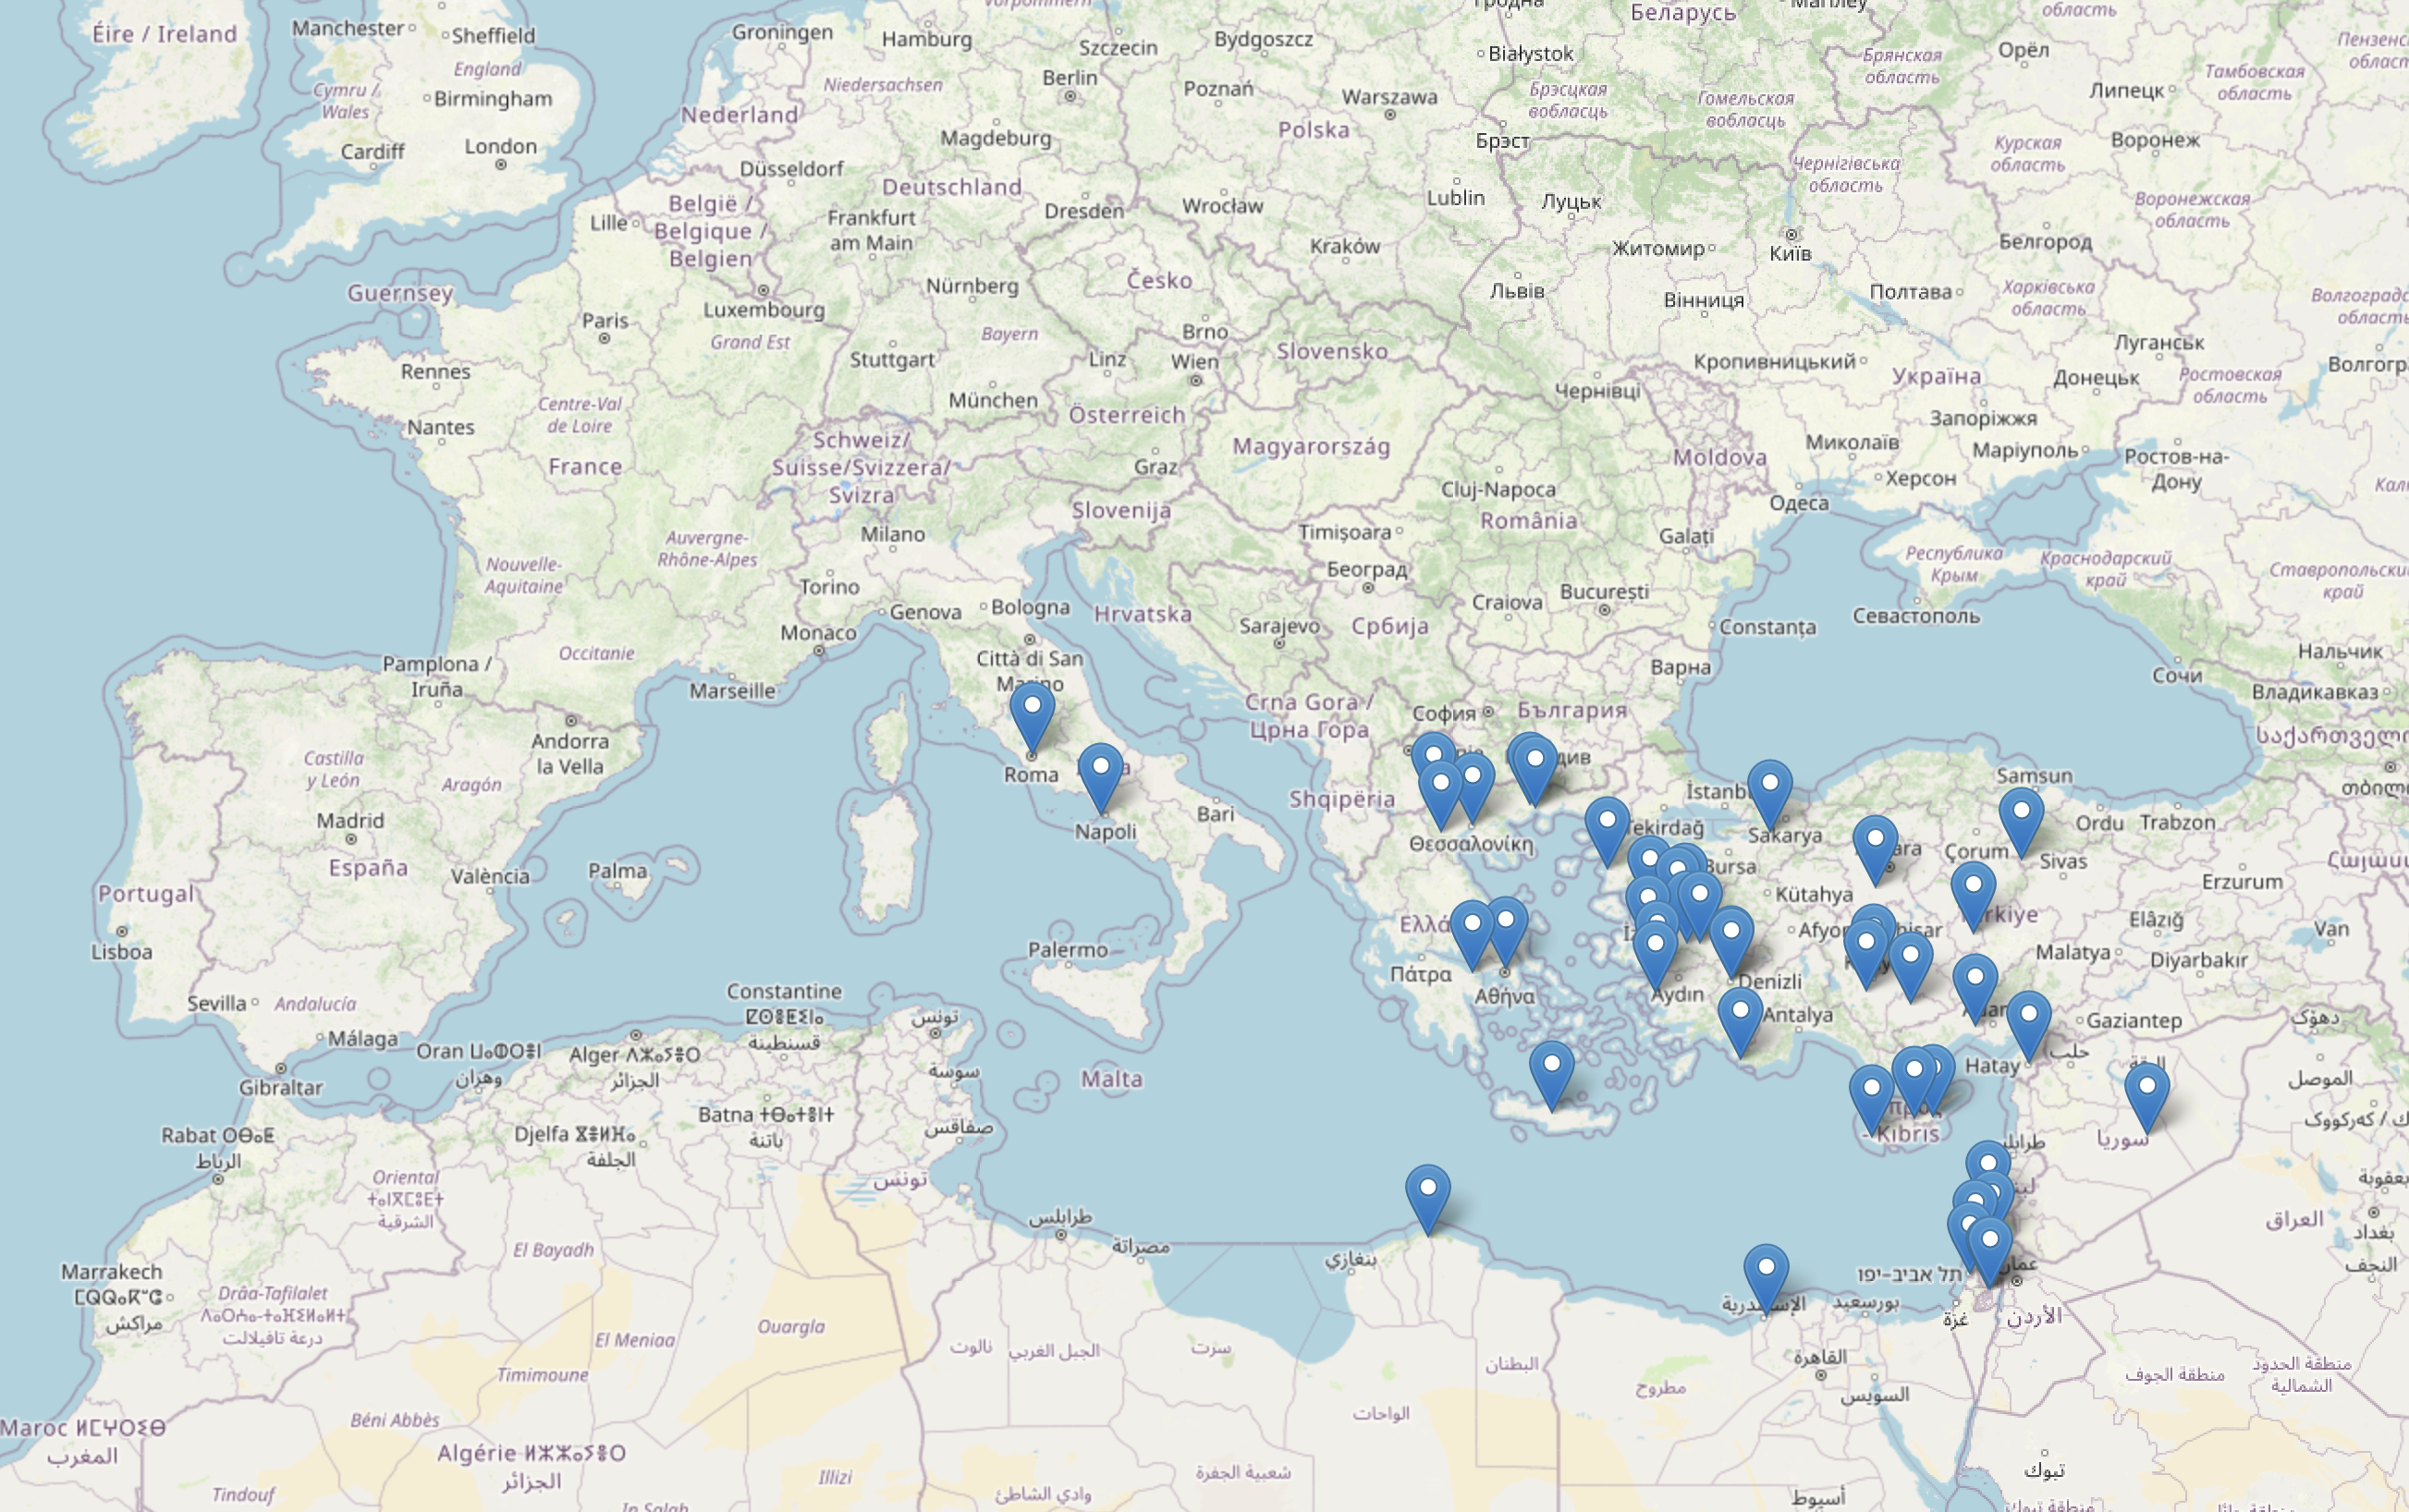
\includegraphics[width=\textwidth, keepaspectratio]{../../assets/locations_map}
    \caption{Mapa wszystkich lokalizacji wymienionych w Dziejach i listach.}
    \label{fig:figure}
\end{figure}

Osoby obeznane geograficznie dostrzegą niemal idealną korelację z granicami wschodniego cesarstwa rzymskiego.
Warto zwrócić uwagę na podróż do Rzymu, która miała zupełnie inny charakter niż pozostałe wyprawy.
\href{https://en.wikipedia.org/wiki/Byzantine_Empire_under_the_Theodosian_dynasty\#/media/File:4KTHEODOSIAN.png}{Mapa Rzymu}

\subsection{Uderzająca statystyka miast wymienionych w Dziejach i listach polega na tym, że wszystkie leżą w dawnym imperium greckim — i nie ma ani jednej wzmianki o mieście w imperium rzymskim, które nie należało wcześniej do imperium greckiego.}\label{subsec:the-striking-statistics-of-the-cities-mentioned-in-the-acts-and-the-epistles-are-that-they-are-all-in-the-former-greek-empire-and-not-one-mention-of-a-city-in-the-roman-empire-that-was-not-part-of-the-former-greek-empire.}

Ten fakt sprawia, że każda teoria uznająca chrześcijaństwo za ruch wyłącznie religijny, a nie polityczny, staje się natychmiast wysoce nieprawdopodobna.

\subsection{Minimalny opór wobec przyjęcia nowej religii.}\label{subsec:minimal-resistance-to-the-acceptance-of-the-new-religion.}

Nowa religia została przyjęta przez masy w dawnym imperium greckim i nie ma ani jednej wzmianki o oporze wobec niej ze strony samych Greków.
Jedyny realny sprzeciw pochodzi od władz świątynnych w Jerozolimie.
Jest to spójne z tezą, że chrześcijaństwo stanowi kontynuację greckiej filozofii imperialnej, którą ludność zhellenizowana już wcześniej akceptowała.

\subsection{Choć religia była tak skuteczna w pozyskiwaniu mas, zachowywała wszystkie elementy konspiracyjności.}\label{subsec:even-though-the-religion-was-so-successful-at-converting-the-masses-it-still-had-all-the-conspiratorial-parts-to-it.}

Pierwsi chrześcijanie używali tajnych symboli, by się rozpoznawać, spotykali się nocą, organizowali wspólne posiłki, posługiwali się zakodowaną ikonografią (ryba, kotwica, chi-rho) i unikali widoczności publicznej ze względu na wrażliwość polityczną.
Zarówno kult Mitry, jak i chrześcijaństwo funkcjonowały jako dyskretne, związkowe bractwa inicjacyjne związane przysięgą — różnica dotyczy treści teologicznej, a nie formy socjologicznej.
Pauline sformułowanie „żołnierze Chrystusa” idealnie wpisuje się w ten konspiracyjno-wojskowy model.

\subsection{Chrześcijaństwo było znacznie bardziej prześladowane niż jakakolwiek inna religia w imperium rzymskim.}\label{subsec:christianity-much-more-prosecuted-than-any-other-religion-in-the-roman-empire.}

Imperium rzymskie było bardzo tolerancyjne wobec innych kultów, a jedynym powodem ich ścigania było uznanie ich za zagrożenie dla państwa.
Chrześcijanie byli prześladowani nie za to, że czcili obcego boga, lecz za odmowę udziału w kulcie cesarskim przy równoczesnym twierdzeniu, że jedynie ich Chrystus jest królem.

Najpierw trzeba zauważyć, że najszerzej znane źródło o wczesnym prześladowaniu chrześcijan — oskarżenie Nerona, jakoby chrześcijanie wzniecili Wielki Pożar Rzymu — jest dziś powszechnie dyskredytowane jako zmyślenie.
Tacyt wspomina w swoim dziele o \emph{Chrestosie}, co było bardzo pospolitym imieniem i niemal na pewno nie odnosi się do Jezusa.
Pisząc po raz pierwszy o chrześcijanach, Tacyt — pięćdziesiąt lat po wydarzeniach — nie zna tej grupy.
To samo dotyczy Pliniusza Młodszego, który w swoim liście do Trajana również nie orientuje się, kim są chrześcijanie.
Gdyby chrześcijan obarczano winą za największą katastrofę w życiu zarówno Tacyta, jak i Pliniusza, byłoby nie do pomyślenia, by o tym nie wiedzieli.

Jednocześnie jednak Piotr został stracony w Rzymie przez ukrzyżowanie, a Paweł — przez ścięcie.
Podobnie jak w przypadku Jezusa, ukrzyżowanie było zarezerwowane dla zbrodni przeciw państwu, buntów i zdrady.
Jako obywatel rzymski Paweł został ścięty za te same przestępstwa.
Jeżeli nie istniały zorganizowane prześladowania chrześcijan, trudno wyjaśnić, dlaczego zarówno Piotr, jak i Paweł zostali zgładzeni w taki właśnie sposób.

\subsection{Określenie „żołnierze Chrystusa” nie pojawia się dosłownie w Ewangeliach, ale występuje wyraźnie w listach Pawła.}\label{subsec:the-phrase-soldiers-of-christ-is-not-used-explicitly-in-the-gospels-but-it-appears-prominently-in-the-pauline-epistles-particularly-in-the-context-of-the-christian-life-being-compared-to-a-military-struggle-or-a-spiritual-battle.}

W świecie rzymskim metafory wojskowe nigdy nie były tylko metaforami.
Autorzy rzymscy używali języka żołnierskiego wobec grup, które składały przysięgi, miały tajne lojalności, utrzymywały wewnętrzną dyscyplinę i działały w komórkach lub bractwach.
Cyceron nazywa spiskowców Katyliny „żołnierzami Katyliny” długo po tym, jak byli nieuzbrojeni (\emph{Filipiki} 13.27).
Józef Flawiusz opisuje zwolenników Judy Galilejczyka jako „zdyscyplinowanych jak żołnierze”, choć nie stanowili regularnej armii (\emph{Dawne Dzieje Izraela} 18.23).
Plutarch opisuje frakcje polityczne jako działające „jak żołnierze”, nawet bez broni (\emph{Żywot Sertoriusza} 26).
Ilekroć ruch był związany przysięgą lub nastawiony na zmianę ustroju, autorzy rzymscy spontanicznie sięgali po język żołnierski, nawet jeśli nie istniała otwarta armia.

Paweł intensywnie korzysta z tego słownictwa: στρατιώτης Χριστοῦ, „żołnierz Chrystusa” (2 Tm 2:3); συστρατιώτης, „współ-wojownik” (Flp 2:25; Flm 2); στρατεία, „kampania wojenna” (1 Kor 9:7; 2 Kor 10:3–4); πανοπλία, „pełna zbroja” (Ef 6:11).
Wszystkie te cztery terminy należą do sfery składania przysięgi, zdyscyplinowanego posłuszeństwa, gotowości do konfliktu i wspólnej walki.
Starożytny słuchacz, słysząc „żołnierze Chrystusa”, nie odbierałby tego jako miłej metafory.
Usłyszałby: to grupa lojalnościowa zorganizowana jak armia.

Rzymskie przesłuchania chrześcijan potwierdzają tę interpretację.
Pliniusz, Tacyt i \emph{Acta Scillitanorum} wielokrotnie zarzucają chrześcijanom nielegalne zgromadzenia, tajne przysięgi, odmowę udziału w kulcie cesarskim i przynależność do \emph{collegium illicitum}.
Rzymianie opisują ich jako grupy związane przysięgą i zdyscyplinowane — znacznie bliższe oddziałom żołnierskim niż dobrowolnym klubom kultowym.
Jeśli chrześcijanie otwarcie posługiwali się językiem żołnierskim, urzędnicy rzymscy traktowali to dosłownie.

Miasta Pawła — Filippi, Korynt, Tesalonika, Efez, Antiochia — wszystkie posiadały stałe lub półstałe garnizony rzymskie.
Kiedy Paweł nazywa zaufanych współpracowników „współ-wojownikami”, nadaje im standardowy rzymski tytuł dowódców komórek wewnątrz zorganizowanego ruchu.
Ma to pełny sens w świecie, w którym Jezus jest królem, królestwo jest realne, lojalność wobec Chrystusa koliduje z lojalnością wobec Cezara, a wierzący działają jak podziemna struktura przygotowująca się do przestawienia ładu politycznego.

\section{Wczesne datowanie Ewangelii może uczynić listy Pawła bardziej wiarygodnymi, ponieważ wydaje się, że Paweł zna przynajmniej jedną z Ewangelii oraz Dzieje Apostolskie.}\label{sec:the-early-dating-of-the-gospels-can-make-the-letters-of-paul-more-plausible-as-it-seems-paul-already-has-the-knowledge-of-at-least-one-of-the-gospels-and-the-acts.}

Wielu badaczy podaje w wątpliwość istnienie Pawła, opierając się na uderzającej sprzeczności w nurcie głównym: autorzy listów Pawłowych zdają się znać Ewangelie i Dzieje, a równocześnie Ewangelie i Dzieje są niemal jednomyślnie datowane na okres \emph{po} listach Pawła.
W tym ujęciu samo istnienie Pawła można ponownie przemyśleć, jeśli przyjmiemy wczesne datowanie Ewangelii i to, że Ewangelia Jana została napisana przez naocznego świadka życia Jezusa.

\subsection{Paweł ledwie wspomina o życiu Jezusa i prawie nigdy go nie cytuje.}\label{subsec:paul-barely-mentions-the-life-of-jesus-and-almost-never-quotes-him.}

Często twierdzi się, że religia Pawła nie jest religią Jezusa, lecz religią o Jezusie.
Uderza brak odniesień do jakichkolwiek nauk Jezusa, do prawa żydowskiego oraz do wydarzeń związanych z życiem i śmiercią Jezusa.
Możemy więc pójść o krok dalej.
Jest to religia skupiona na odnowieniu królestwa Bożego poprzez przywrócenie urzędu Christosa, prawowitego króla królestwa Bożego.
Dlatego dla Pawła i wszystkich wczesnych chrześcijan chodziło przede wszystkim o przywrócenie Chrystosa, a nie o nauczanie konkretnego Jezusa Chrystusa.
Chodziło o to, że Bóg ponownie pośle króla, który odnowi imperium greckie — królestwo Boże — pod przewodnictwem Christosa, prawowitego ziemskiego króla królestwa Bożego.

\subsection{Używanie tego języka konspiracyjnego jasno zadziałało.}\label{subsec:using-this-conspiratorial-language-clearly-worked}

Rzym nawet nie zorientował się, że celem nowej religii jest przywrócenie Wschodniego Imperium, dopóki to faktycznie nie nastąpiło.

\subsection{10.
Aleksandria była stolicą imperium greckiego i centrum świata hellenistycznego, a jednak nie ma żadnych misji ani listów skierowanych do Aleksandrii.}

\label{subsec:alexandria-was-the-capital-of-the-greek-empire-and-the-center-of-the-hellenistic-world-and-yet-there-are-no-missions-or-letters-to-alexandria.}

Nieobecność Aleksandrii w Nowym Testamencie jest uderzająca, zwłaszcza jeśli uwzględnić jej znaczenie.
Aleksandria została z tekstu usunięta, choć była miastem pochodzenia Apollosa oraz niektórych innych towarzyszy Pawła, takich jak Marek, Demas i Łukasz.
To przemilczenie najlepiej wyjaśnić jako celowe wymazanie, właśnie dlatego, że Aleksandria była już centrum ruchu.
Tak jak Stary Testament w dużej mierze pomija imperium Ptolemejskie mimo jego centralnego znaczenia, tak Nowy Testament minimalizuje rolę Aleksandrii, jednocześnie zakładając jej przywództwo.

\section{Dzieje Apostolskie}\label{subsec:acts-of-the-apostles}

Nazywają się Dzieje \emph{Apostolskich}, a nie dzieje uczniów.
Apostołowie wykonują pracę imperialną: ogłaszają wszystkim narodom imperium wolę Boga-Króla.

\subsection{10.
Dzieje rozpoczynają się od królewskiej intronizacji}\label{subsec:acts-opens-with-a-royal-enthronement}

Dz 1:6 --- „Panie, czy w tym czasie odbudujesz królestwo Izraela?”.
To nie jest pytanie duchowe.
Zakłada, że Jezus rości sobie prawo do politycznego królowania.
Twoja teoria: Jezusa postrzegano jako prawowitego monarchę odnowionego królestwa — następcę tronów herodiańskich lub hasmonejskich w ramach greckich ideałów imperialnych.

\subsection{10.
Jezus zostaje wzięty do nieba jak cesarz}\label{subsec:jesus-is-taken-up-like-an-emperor}

Dz 1:9–11 --- Wniebowstąpienie naśladuje sceny apoteozy (np. Aleksandra, cesarzy rzymskich).
Przedstawia Jezusa w kategoriach imperialnych, jako wyniesionego na tron w niebie — jak boskiego cesarza.
To dokładnie odpowiada ujęciu, że chrześcijaństwo dotyczyło lojalności wobec „Chrystusa-Cesarza”.

\subsection{10.
Scena Pięćdziesiątnicy naśladuje inaugurację imperialną}\label{subsec:the-pentecost-scene-mimics-an-imperial-inauguration}

Dz 2 --- Cud wielojęzyczności i masowego nawrócenia odzwierciedla imperialny ideał zjednoczenia narodów pod jednym boskim królem.
Język „języków” ma wymiar polityczny: przesłanie cesarza jest przeznaczone dla wszystkich narodów.

\subsection{10.
Dz 5: proces apostołów}\label{subsec:acts-5-the-trial-of-the-apostles}

Gamaliel przywołuje wcześniejszych przywódców rewolucyjnych — Teudasa i Judę Galilejczyka.
Potwierdza w ten sposób, że mesjańskie bunty miały charakter polityczny i że ruch Jezusa był postrzegany w podobnych kategoriach.

\subsection{10.
Mowa Szczepana w Dz 7 jest anty-świątynna}\label{subsec:stephens-speech-in-acts-7-is-anti-temple}

Szczepan atakuje Świątynię i tradycję Mojżeszową, nawiązując do krytyki legalizmu żydowskiego u Filona i myślicieli stoickich.
Wspiera to pogląd, że wczesne chrześcijaństwo odrzucało religię Mojżeszową i było bliższe filozoficznemu monoteizmowi.

\subsection{10.
Dzieje kończą się bez rozwiązania akcji}\label{subsec:acts-ends-without-resolution}

Księga kończy się w Rzymie, gdzie Paweł swobodnie głosi „królestwo Boże”.
Brakuje narracyjnego finału, ponieważ prawdziwe przesłanie brzmi: imperium jest już chrześcijańskie.
Zakłada to istniejącą wcześniej publiczność, która widzi chrześcijaństwo jako siłę polityczno-teologiczną.

\subsubsection{Jakub Sprawiedliwy}\label{subsec:james-the-just}

\subsection{Jakub Sprawiedliwy również napisał list do wszystkich narodów.}\label{subsec:james-the-just-also-wrote-an-epistle-to-all-nations.}

Był bratem Jezusa i kolejnym w linii dziedziczenia tronu.
Podobnie jak Jezus Chrystus Zbawca, Jakub nosił tytuł królewski: Sprawiedliwy.

Jakub Sprawiedliwy również napisał list do wszystkich narodów, włączony do Nowego Testamentu.
Jakub, podobnie jak Jan, odwołuje się do tego samego rozumienia Logosu co Filon z Aleksandrii.
Styl retoryczny Jakuba — moralna diatryba z wyimaginowanymi rozmówcami, wezwania w trybie rozkazującym, żywe przykłady — należy do tego samego hellenistycznego nurtu filozoficznej nauki moralnej, który przejął Filon.

Po grecku Jk 1:21 brzmi:
„Διὸ ἀποθέμενοι πάσαν ἀκαθαρσίαν καὶ περισσείαν κακίας ἐν πραΰτητι δέξασθε τὸν ἐμφυτον λόγον, ὃς δύναται σῶσαι τὰς ψυχὰς ὑμῶν.”
Transliteracja: „Dio apothemenoi pasan akatharsian kai perisseian kakias en prautēti dexasthe ton emphuton logon, hos dynatai sōsai tas psychas hymōn.”
Przekład dosłowny: „Dlatego, odrzuciwszy wszelką nieczystość i nadmiar zła, w łagodności przyjmijcie wszczepione słowo, które może zbawić wasze dusze.”

List Jakuba jest napisany wyrafinowaną literacką koine, z użyciem złożonych zdań podrzędnie złożonych, szerokiego i częściowo twórczego słownictwa (zawiera ponad sześćdziesiąt słów unikatowych w Nowym Testamencie) oraz technik retorycznych hellenistycznej diatryby moralnej — paronomazji, aliteracji, personifikacji i gwałtownych pytań retorycznych.
Taki poziom greki trudno pogodzić z analfabetą-parobkiem wiejskim i wskazuje raczej na postać osadzoną w wykształconych, greckojęzycznych sieciach wschodniego basenu Morza Śródziemnego, czy to dzięki własnej formacji, czy we współpracy z biegłym skrybą.

\subsubsection{Listy Jana}\label{subsec:the-epistles-of-john}

\subsection{Obalenie istniejących modeli}\label{subsec:a-disproof-of-existing-models}

Literatura naukowa zwykle wyjaśnia powstanie chrześcijaństwa w ramach jednego z trzech modeli: misyjnej dyfuzji, żydowskiej sekty lub konkurencji kultów imperialnych.
Wszystkie trzy zakładają, że chrześcijaństwo rozpoczęło się jako mała grupa religijna i stopniowo rozszerzało poprzez procesy organiczne.
Rzeczywiste dane pokazują, że to założenie jest niemożliwe.

\textbf{1. Model misyjnej dyfuzji (Harnack, Stark i in.).}
Model ten wyobraża sobie apostołów podróżujących od miasta do miasta, nawracających domy i zakładających lokalne wspólnoty, które następnie rosły z czasem.
Przewiduje on: (a) stopniowe rozprzestrzenianie się po regionach, (b) nierównomierną recepcję, (c) wielojęzyczną dokumentację oraz (d) ciągły wzrost w II wieku.
\emph{Obserwacja:} nagła sieć kościołów w każdym większym polis greckiego Wschodu, wyłącznie w języku greckim, po czym następuje stulecie stagnacji.
\emph{Wniosek:} model nie jest w stanie tego wyjaśnić.
Stopniowa dyfuzja nie daje w efekcie natychmiastowej obecności w całym imperium, a potem ciszy.

\textbf{2. Model żydowskiej sekty (Eisenman, Sanders, Vermes i in.).}
Model ten opisuje chrześcijaństwo jako mesjańską reformę wewnątrz judaizmu, która dopiero później otworzyła się na pogan.
Przewiduje: (a) najwcześniejsze pisma w języku aramejskim lub hebrajskim, (b) oparcie na prawie Mojżeszowym i tradycji świątynnej, (c) ekspansję poprzez diasporę synagogalną oraz (d) późniejsze tłumaczenia na grekę.
\emph{Obserwacja:} ani jednego listu po aramejsku czy hebrajsku, brak rozprzestrzeniania się przez synagogi, wrogość wobec prawa Mojżeszowego i powszechna korespondencja w języku greckim.
\emph{Wniosek:} oczekiwane żydowskie ramy są całkowicie nieobecne.
Ruch jest grecki i imperialny od samego początku.

\textbf{3. Model konkurencji kultów imperialnych (Friesen, Harland i in.).}
Model ten ujmuje chrześcijaństwo jako kolejny kult miejski konkurujący na rzymskim rynku religijnym.
Przewiduje: (a) stopniowe przyjmowanie zarówno na łacińskim Zachodzie, jak i na greckim Wschodzie, (b) lokalną różnorodność praktyk, (c) synkretyzm z kultem cesarskim oraz (d) powolny wzrost od prywatnych stowarzyszeń do kultu publicznego.
\emph{Obserwacja:} brak ekspansji na łaciński Zachód, brak losowego rozproszenia po miastach rzymskich, za to pełne pokrycie dawnego imperium greckiego z jednolitym roszczeniem jednego królewskiego Chrystosa.
\emph{Wniosek:} dane obalają ten model.
Zamiast rozproszonej konkurencji kultów, widzimy wzorzec spójny i scentralizowany.

\textbf{Ostateczna ocena.}
Każdy z modeli alternatywnych się załamuje.
Ich przewidywania nie tylko „słabo pasują” — są całkowicie nie do pogodzenia z rzeczywistymi świadectwami.
Jest więc pewne, że wczesne chrześcijaństwo nie było produktem misyjnego wzrostu, żydowskiego sekciarstwa ani konkurencji kultów.
Kościoły nie były świeżo zakładanymi zgromadzeniami, lecz kontynuującymi działalność \textit{ekklesiami} świata greckiego, przeorganizowanymi pod panowaniem Christosa.
Sekwencja wydarzeń — brak obecności, natychmiastowe pokrycie imperialne, potem długotrwała stagnacja — dopuszcza tylko jedno wyjaśnienie: kontynuację imperium greckiego pod nową proklamacją królewską.

\subsection{Korpus Nowego Testamentu}\label{subsec:the-corpus-of-the-new-testament}

Co tak naprawdę wchodzi w skład Nowego Testamentu i jak rozkłada się to na cztery bieguny imperialne, które zidentyfikowaliśmy?
Poniżej czynimy tę mapę jawną \emph{oraz} kotwiczymy ją w konkretnych starożytnych świadectwach, zwłaszcza w odniesieniu do listów i wczesnych twierdzeń o autorstwie.
Warto podkreślić: w starożytności przypisania czterech kanonicznych Ewangelii \textit{Mateusz, Marek, Łukasz, Jan} są jednomyślnie podtrzymywane przez Ojców.
Nie zanotowano dla nich żadnych alternatywnych apostolskich imion.

\subsection{Świadectwa patrystyczne (autorstwo w starożytności).}

Przed połową III wieku obraz jest spójny.
\textbf{Papias} (przez Euzebiusza, \textit{Hist.\ Eccl.} 3.39) — Marek pisał jako tłumacz Piotra.
Mateusz zebrał \textit{logia}.
\textbf{Ireneusz} (\textit{Adv.\ Haer.} 3.1.1) — wprost wylicza i broni czterech: Mateusza, Marka, Łukasza (towarzysza Pawła) i Jana.
\textbf{Fragment Muratoriański} (koniec II w.) nazywa Łukasza i Jana trzecim i czwartym ewangelistą i rozpoznaje korpus Pawłowy.
\textbf{Klemens Aleksandryjski} i \textbf{Orygenes} powtarzają te przypisania.
\textbf{Euzebiusz} później podsumowuje je jako powszechnie przyjęte.
Co do listów: \textbf{1 List Klemensa} (ok. 96 r.) cytuje 1 List do Koryntian.
\textbf{Ignacy} (ok. 110 r.) zakłada istnienie kościołów pawłowych i ich języka.
\textbf{Polikarp} (ok. 135 r.) cytuje lub parafrazuje wiele listów Pawła i 1 List Piotra.
\textbf{Ireneusz} korzysta z 1–2 Listu Piotra, 1 Listu Jana i Listu Jakuba jako pism apostolskich.
Dyskusje nad autorstwem Listu do Hebrajczyków i późnością 2 Listu Piotra pojawiają się dopiero później.
Kluczowe jest to, że nie ma wczesnych kontrprzypisań \emph{czterech Ewangelii} do innych imion.

\subsection{Papirologia i wczesny obieg (migawka).}

\textbf{P\textsuperscript{46}} (ok. 200 r.) zawiera zbiór listów Pawła (Rz, 1–2 Kor, Ga, Ef/Kol, Flp, 1 Tes, Hbr), pokazując, że listy krążyły już jako korpus.
\textbf{P\textsuperscript{66}} (ok. 200 r.) i \textbf{P\textsuperscript{75}} (początek III w.) to główne wczesne świadectwa Ewangelii Jana (oraz Łukasza/Jana).
\textbf{P\textsuperscript{9}} (III w.) zachowuje fragment 1 Listu Jana z Oksyrynchos.
\textbf{P\textsuperscript{72}} (III/IV w.) zawiera 1–2 List Piotra i List Judy.
\textbf{P\textsuperscript{13}} (III w.) — List do Hebrajczyków.
\textbf{P\textsuperscript{45}} (III w.) — Ewangelie/Dzieje.
Świadectwa te potwierdzają wczesny obieg i naturalne klastrowanie (zestaw Pawłowy; Piotrowy/Judy; Janowy), które odzwierciedla naszą czterobiegunową architekturę.
Egipskie miejsca znalezienia odzwierciedlają stronniczość zachowania materiału.
\emph{Kompozycyjne} skupiska nadal odpowiadają mapie imperialnej.

\subsection{Cztery ocalałe greckie światy kulturowe po Aleksandrze}

Istnienie czterech kanonicznych Ewangelii nie było późniejszym redakcyjnym przypadkiem ani teologicznym kompromisem.
Odzwierciedla coś znacznie starszego i głębszego: sam wschodni basen Morza Śródziemnego był ustrukturyzowany w cztery wielkie światy kulturowe, które przetrwały w niezmienionej formie od czasu rozpadu imperium Aleksandra.
Ewangelie powstały wewnątrz tego czteroczłonowego świata, a ich różnice odzwierciedlają właśnie te cztery ocalałe greckie sfery kulturowe.

Gdy imperium Aleksandra się rozpadło, nie rozkruszyło się na dziesiątki równorzędnych państw; niemal natychmiast skrystalizowało się w cztery dominujące regiony dynastyczne, z których każdy stał się samowystarczalnym ekosystemem kulturowym, z własnymi instytucjami, własnym idiomem greckim i własną pamięcią polityczną.
Nie były to jedynie królestwa w sensie politycznym; były to całe cywilizacyjne światy, każdy na tyle rozległy, by kształtować życie milionów ludzi, i na tyle stabilny, by trwać przez stulecia, nawet po zniknięciu samych dynastii.
Każde ważniejsze miasto, każdy lud i każdy system edukacyjny we wschodnim basenie Morza Śródziemnego należał do jednego z tych czterech światów.

Ptolemejska Egipt zbudował najbardziej intelektualnie ambitną kulturę grecką starożytności.
Aleksandria pozostała bezdyskusyjnym centrum badań, żydowsko–greckiej syntezy filozoficznej, produkcji tekstów i spekulacji metafizycznej, nawet po tym jak August przyłączył Egipt do imperium.
Jej instytucje przeżyły dynastię: Muzeum, akademie filozoficzne, kultura skrybów oraz charakterystycznie aleksandryjski styl greki pojęciowej przetrwały w stanie nienaruszonym.
To właśnie ten świat wydał teologię Logosu, dualizmy platońskie, dialogi objawieniowe i słownik metafizyczny, które znamionują Ewangelię Jana.
Jan nie jest anomalią; to głos judaizmu aleksandryjskiego, mówiącego po grecku w swoim własnym intelektualnym rejestrze.

Seleucka Syria, z Antiochią jako stolicą, rozwinęła zupełnie inne greckie środowisko: grecką metropolię na skraju aramejskojęzycznego zaplecza.
Rzeczywistość językowa tego regionu była stabilna i jednoznaczna — greka w miastach, aramejski na prowincji — co tworzyło naturalny, niewymuszony bilingwizm.
Krótkie rozkazy, przezwiska, okrzyki, formuły uzdrowień i pograniczne zwroty nieustannie przechodziły z jednego języka do drugiego.
Dokładnie taki wzorzec zachowuje się w aramejskich zwrotach Marka.
Nie są to relikty galilejskiego Jezusa; to nawyki kodowego przełączania się językowego greckiego autora z Antiochii, piszącego wewnątrz syryjsko–seleuckiego świata dwujęzycznego.
Heroiczny styl pogranicza, urywana narracja, epicko–mimetyczna struktura i mieszanka greki z aramejskim doskonale pasują do Antiochii, a wcale do Galilei.

Królestwo Judei, stworzone przez Hasmoneuszy na długo przed wejściem Rzymu do regionu, było projektem dużego, spójnego, politycznie ambitnego ludu, zdeterminowanego, by rządzić sobą samym.
Nie było wytworem Rzymian.
Zdobyli niezależność, ponieważ w momencie załamania władzy Seleucydów byli wystarczająco silni i dobrze zorganizowani, by stworzyć własną dynastię i zachować własne tradycje w obrębie greckiej oikoumene.
Herodiańscy następcy kontynuowali ten świat w innym tonie, ale blok kulturowy trwał: region z własnymi szkołami prawa, własną pamięcią dynastyczną, własnymi sporami o legitymizację i własną tożsamością w ramach greckiej kultury politycznej.
Ewangelia Mateusza odzwierciedla to środowisko z niezwykłą precyzją: genealogia dynastyczna, argumentacja prawno–egzegetyczna, formuły wypełnienia proroctw i judejska teologia polityczna wyrażona po grecku, a nie egejski styl retoryczny, ani aleksandryjski styl metafizyczny, ani syryjski styl bilingwalny.

Świat Antygonidów — Macedonia, Grecja i basen Morza Egejskiego — był czwartym wielkim postaleksandryjskim kręgiem kulturowym.
Nawet po zgnieceniu samej dynastii instytucje, które zbudowała, przetrwały w niezmienionej formie.
Gimnazja, szkoły retoryki klasycznej, zgromadzenia polis, dekrety honorowe, tradycja historiografii elit i system edukacyjny greckiego lądu oraz zachodniej Azji Mniejszej wszystkie wywodziły się z fundamentów antygonidzkich.
W I wieku Efez stał się faktyczną metropolią całego tego regionu: największym, najbogatszym, najbardziej „instytucjonalnie greckim” miastem świata egejskiego.
To właśnie ten krąg kulturowy wydał Saloniki, Filippi, Korynt i szerszą, miejską sieć pawłową.
To także sfera odzwierciedlona w grece Łukasza: wyszlifowany proem historiograficzny, precyzja administracyjna, słownictwo żeglarskie, terminologia miejska i struktura retoryczna nauczana w gimnazjach egejskich.
Łukasz nie pisze „ogólnej” greki; pisze greką klasycznego centrum edukacyjnego całego Morza Śródziemnego.

Te cztery światy były jedynymi realnymi, wielkoskalowymi podziałami kulturowymi greckiego Wschodu.
Każdy inny podział jest sztuczny.
Każdy region podpadał pod któryś z tych bloków.
Ich kultury instytucjonalne przetrwały długo po tym, jak dynastie przestały rządzić.
Pod rzymską administracją te cztery światy nadal istniały jako fakty kulturowe: Aleksandria myślała jak Ptolemeusze, Antiochia jak Seleucydzi, Jerozolima jak jej rodzima dynastia, a miasta egejskie jak świat Antygonidów.

Dlatego właśnie różnorodność Ewangelii wreszcie nabiera historycznego sensu.
Każda Ewangelia nie jest tylko portretem teologicznym; jest wytworem jednego z tych czterech wielkich ekosystemów kulturowych.
Jan przemawia z Aleksandrii.
Marek przemawia z Antiochii.
Mateusz przemawia z Judei.
Łukasz przemawia ze świata egejskiego.
Czterokrotna Ewangelia nie jest przypadkiem powstania kanonu; jest literacką mapą czterech ocalałych kultur greckich wschodniego basenu Morza Śródziemnego.
Sama struktura czterokrotna jest jednak starsza niż Aleksander.

\subsection{Cztery symbole królewskie sprzed Aleksandra}

Czteropolowa mapa, która kształtuje Ewangelie, nie została wymyślona w epoce hellenistycznej.
Czytelnik natychmiast zauważy, że Ezechiel prorokował w VI wieku p.n.e., na długo przed rozbiciem imperium Aleksandra na Ptolemeuszy, Seleucydów, Hasmoneuszy i Antygonidów.
Ten dystans chronologiczny nie stanowi problemu; jest kluczem.
Widzenie Ezechiela należy do świata, w którym Bliski Wschód używał czterech symboli królewskich od ponad tysiąca lat.
Symbole te nie były ozdobą.
Były oficjalnymi insygniami państwowymi, znakami wojskowymi, ikonami świątynnymi i emblematami królewskimi czterech wielkich sfer kulturowych, które poprzedzały wszystkie późniejsze imperia.
Gdy Ezechiel widzi lwa, wołu, orła i człowieka, opisuje ugruntowaną polityczną i kosmologiczną gramatykę starożytnego Bliskiego Wschodu — sposób, w jaki królestwa przedstawiały władzę.
Te cztery emblematy stoją w centrum politycznej teologii regionu na długo przed Ewangeliami i na długo przed rządami hellenistycznymi.

Przez ponad dwa tysiące lat przed Ezechielem symbolem królewskości Egiptu był koronowany sokół Horusa, umieszczony nad imieniem królewskim w każdej kartuszy.
Każdy faraon od Starego Państwa w górę był explicite tytułowany „Horus”, a ptak–sokół pojawiał się na znakach wojskowych, fasadach pałacowych, świątyniach grobowych, chorągwiach wojskowych i w biżuterii królewskiej.
W Okresie Późnym — za życia samego Ezechiela — sokół pozostawał oficjalnym emblematem egipskiej suwerenności, widocznym w ikonografii tronu, w szatach kapłańskich i na reliefach monumentalnych.
Dlatego oblicze orła u Ezechiela jest natychmiast rozpoznawalne: przywołuje wschodni symbol boskiego królowania, stworzenie, które dosłownie spoczywa na głowie każdego faraona jako duet ureus–Horus.
Gdy Ptolemeusze później rządzą Egiptem, przyjmują Orła Zeusa, będącego po prostu greckim odpowiednikiem sokoła Horusa: królewskiego ptaka nieba, emblemat suwerenności.
Symbol ten jest tak dominujący, że staje się rzymskim orłem legionowym, a przez Rzym przechodzi w emblemat Bizancjum, Niemców, Rosjan, Polaków, Amerykanów i republik arabskich.
Orzeł jest najstarszym nieprzerwanym symbolem królewskim wschodniego basenu Morza Śródziemnego i politycznym obliczem wschodniego kwadrantu starożytnego świata.

We wschodnim Lewancie — świecie fenickim i aramejskim — wół był najwyższym symbolem władzy państwowej przez co najmniej tysiąc lat przed Aleksandrem.
Wół był żywym emblematem Baala i Hadada, królewskiego boga burzy tego regionu, który w tekstach ugaryckich z XIII–XII wieku p.n.e. zasiada na tronie na grzbiecie wołu, włada deszczem i legitymizuje królów.
Fenickie świątynie w Byblos, Tyrze i Sydonie wystawiały przy bramach brązowe woły; miasta aramejskie rzeźbiły posągi wołów jako figury strażnicze; królewskie pieczęcie w całym Kanaanie przedstawiają bóstwa o głowach wołów przekazujące władzę królom.
Gdy Biblia opisuje, że Izrael buduje złotego cielca, nie mówi o przypadkowym bożku — opisuje oficjalnego fenickiego boga państwowego, królewski emblemat całego systemu monarchii nadbrzeżnych.
W czasach Ezechiela wół jest już rozpoznawalnym symbolem zachodniego kwadrantu, rolniczo–morskiego świata rządzonego przez bogów burzy.
Gdy Seleucydzi później budują swoje imperium na tym samym obszarze, przyjmują hybrydę wołu, konia i rogatej ikonografii mocy, która kontynuuje ten liczący tysiąclecia emblemat władzy.
Ox face Ezechiela nie jest więc zwierzęciem wybranym losowo; to polityczny symbol całego zachodniego bloku lewantyńsko–syryjskiego.

Na długo przed Ezechielem lew stał się kanonicznym emblematem królewskości w całym wnętrzu świata zachodniosemickiego, od Kanaanu i Moabu po Izrael i Judę.
Pałace asyryjskie pokrywają się niekończącymi się reliefami polowań na lwy, ponieważ lew symbolizował królewską dominację, a Babilon wznosi całe aleje lwów na potrzeby rytuałów państwowych.
Biblijny „Lew Judy” nie jest uroczą metaforą: to judejski emblemat państwowy poświadczony w ideologii królewskiej co najmniej od czasów Dawida, wzmocniony w błogosławieństwie Judy w Rdz 49 i wsparty ikonografią lwa na pieczęciach judejskich, dzbanach magazynowych i architekturze monumentalnej.
Potęga lwa nad pustynią, jego drapieżna gwałtowność i związek z królewskim podbojem uczyniły go naturalnym symbolem południowego kwadrantu: wyżyn zachodniosemickich i pustyń pogranicza.
W świecie Ezechiela lew pełni już funkcję identyfikatora królewskiej linii Izraela, tak jak sokół identyfikuje Egipt, a wół Fenicję.
Lew Ezechiela reprezentuje więc południową kulturę królewską na symbolicznej mapie Bliskiego Wschodu.

Czwarty symbol — człowiek — nie ma być słaby ani neutralny.
To człowiek heroiczny, postać dominująca w sztuce greckiej od epoki brązu.
Freski i kratery mykeńskie ukazują wojowników w hełmach; ceramika okresu geometrycznego przedstawia szeregi hoplitów; rzeźba archaiczna rozwija kurosa jako idealnego obywatela–wojownika; a klasyczne Ateny, Sparta i Macedonia czynią z uzbrojonej postaci ludzkiej podstawowy emblemat tożsamości obywatelskiej.
Świat grecki jest jedynym blokiem kulturowym Bliskiego Wschodu, którego symbol suwerena jest jawnie antropiczny: Achilles, Ajas, Herakles, Perseusz, Tezeusz i ostatecznie obywatel–hoplita.
Przez co najmniej siedem stuleci przed Ezechielem teologia polityczna świata egejskiego buduje się wokół człowieka–herosa, a nie zwierzęcego bóstwa.
Dlatego czwarta twarz Ezechiela — ludzka — należy do północnego kwadrantu, gór i miast–państw Anatolii i Grecji.
Gdy Aleksander rozszerza Grecję w imperium, nie tworzy tej tożsamości; globalizuje to, co już było ludzkim, heroicznym emblematem greckiego panowania.

W czasach, gdy Ezechiel pisze w VI wieku p.n.e., te cztery insygnia dominują w regionie już od ponad tysiąca lat: sokół jako symbol królewskości Egiptu, wół jako znak władzy Fenicji i Syrii, lew jako emblemat królewski Judy i świata zachodniosemickiego oraz człowiek–heros jako znak państw wojowniczych Anatolii i Grecji.
Jego czterotwarzowe stworzenie jest najstarszą zachowaną literacką reprezentacją czteroczłonowego świata bliskowschodniego, łączącą cztery symbole królewskie, cztery bloki kulturowe, cztery wiatry, czterech nosicieli tronu i czteroczłonową strukturę kosmosu.
Gdy Kościół pierwotny później mówi, że Ewangelia musi być czterokrotna, ponieważ świat jest czterokrotny, nie popada w mistykę.
Przypomina sobie tę starożytną symboliczną architekturę — taką, która poprzedza Aleksandra, poprzedza monarchię Izraela i poprzedza samego Ezechiela.
A gdy cztery kanoniczne Ewangelie trafiają w ręce Aleksandrii, Judei, Syrii i świata egejskiego, wchodzą bezpośrednio w czterokwadrantowy system świata, który był wizualnie i politycznie definiowany przez co najmniej tysiąc lat przez sokoła, wołu, lwa i herosa.

\subsection{Dlaczego Ireneusz się nie mylił}

Najwcześniejszym chrześcijaninem, który wyjaśnia, dlaczego istnieją cztery Ewangelie, jest Ireneusz, i podaje on powód, z którego niemal wszyscy dziś kpią: Ewangelie odpowiadają czterem istotom żyjącym — lew, wół, orzeł, człowiek — tym samym czterem istotom z Ezechiela i Apokalipsy.
Uczeni odrzucają to jako numerologię.
Traktują je jako mistyczną ozdobę albo prymitywną symbolikę.
Ale takie odrzucenie jest całkowicie powierzchowne.
Ireneusz nie wybiera zwierząt na chybił trafił.
Czerpie z sztywnej, odziedziczonej kosmologii czterech kierunków — tej samej symbolicznej architektury, której używa starożytna literatura apokaliptyczna — a ta czterostronna struktura jest dokładnie sposobem, w jaki świat śródziemnomorski po Aleksandrze był faktycznie podzielony.
Język symboliczny Ireneusza nakłada się bezpośrednio na realną rzeczywistość geopolityczną.

Ireneusz nie był osamotniony.
Schema czterech stworzeń przenika całą tradycję patrystyczną.
Apokalipsa jest pierwszym chrześcijańskim tekstem, który podejmuje wizję tronu z Księgi Ezechiela i czyni ją centralnym elementem chrześcijańskiej kosmologii: Jan opisuje cztery istoty żyjące „pośrodku tronu i dokoła tronu” (Ap 4,6–8), każdą z inną twarzą — lwa, cielca, człowieka, orła — śpiewające bez wytchnienia Trisagion, dokładnie tak jak cherubini Ezechiela wyznaczali obecność chwały Boga.
Już w Nowym Testamencie czterokrotna istota Ezechiela staje się częścią chrześcijańskiej gramatyki kosmosu i tronu, a nie marginalną ciekawostką.

Pod koniec II wieku Ireneusz czyni tę gramatykę explicite i kanoniczną.
W \textit{Against Heresies} 3.11.8 bierze istoty żyjące z Apokalipsy 4,7 i odczytuje je jako figury całej „ekonomii” Syna Bożego, po czym stwierdza wprost, że „istoty żyjące są czteroformne, Ewangelia jest czteroformna i droga, którą kroczył Pan, jest czteroformna”.
Dla Ireneusza nie chodzi o ładną alegorię, ale o konieczność: Kościół jest rozproszony po czterech wiatrach, świat ma cztery strefy i cztery główne wiatry, a zatem jeden Chrystus musi być głoszony w formie czterokrotnej, jeśli orędzie ma odpowiadać strukturze stworzenia.

Pisarze III wieku wzmacniają tę logikę.
Orygenes, w homiliach do Ezechiela i Łukasza, traktuje liczbę cztery jako immanentną tradycji Ewangelii, wiążąc ją z czterema rzekami Edenu, czterema wiatrami i czterema krańcami ziemi, i po prostu zakłada, że istoty Ezechiela i Jana dostarczają podstawowego schematu tego, jak jeden Chrystus może zostać przedstawiony w wielu, niekonkurujących formach.
Wiktoryn z Patawii, najwcześniejszy zachowany komentator Apokalipsy, jest jeszcze bardziej bezpośredni: komentując Apokalipsę 4 pisze, że „cztery istoty żyjące to cztery Ewangelie” i przypisuje każdej stworzonej istocie jednego ewangelistę, nalegając przy tym, że razem otaczają tron i śpiewają Trisagion.
Na tym etapie identyfikacja jest już ustalona: ilekroć prawowierni chrześcijanie czytają tron z Apokalipsy, widzą wokół niego rozchodzącą się kanoniczną czterokrotną Ewangelię.

Teologia łacińska IV i V wieku przejmuje to i buduje na tym ortodoksję.
Augustyn poświęca cały rozdział w \textit{De Consensu Evangelistarum} „czterem istotom żyjącym w Apokalipsie, które zostały uznane za trafne figury czterech ewangelistów”, przyjmuje identyfikację jako oczywistą i debatuje jedynie nad tym, które stworzenie najlepiej odpowiada któremu ewangeliście.
Dla Augustyna tetramorf oznacza, że ewangeliści różnią się, a zarazem są zgodni, tak jak cztery oblicza mogą należeć do jednego rydwanu–tronu: struktura czterech nie jest przypadkiem przetrwania rękopisów, lecz znakiem, że Duch rozdzielił jedną rzeczywistość chrystologiczną na cztery komplementarne perspektywy.
Hieronim w swoich przedmowach i komentarzu do Mateusza standaryzuje dobrze nam dziś znany zachodni przydział — człowiek dla Mateusza, lew dla Marka, wół dla Łukasza, orzeł dla Jana — i scala go z kolejnością w Wulgacie, która zdominuje sztukę i liturgię średniowiecza.
Późniejsi pisarze łacińscy, tacy jak Chromacjusz czy Raban Maur, po prostu powtarzają ten schemat: cztery istoty żyjące, cztery wiatry, cztery krańce ziemi, czterej ewangeliści, jeden tron.

Kluczowe spostrzeżenie jest takie, że wszyscy ci autorzy nie zgadzają się w szczegółach, które zwierzę odpowiada której księdze, ale absolutnie zgadzają się, że musi być cztery i tylko cztery.
Ireneusz, Wiktoryn, Augustyn, Hieronim i Atanazy dziedziczą różne lokalne tradycje parowania zwierzę–ewangelista, ale żaden z nich nawet nie rozważa piątej Ewangelii ani redukcji do jednej czy dwóch; czterokrotność jest traktowana jako kosmologiczna, a nie redakcyjna.
Gdy odwołują się do Ezechiela i Apokalipsy, przywołują starożytne bliskowschodnie przekonanie, że sam świat jest czteroczęściowy, strzeżony i reprezentowany przez cztery żywe moce, a tron prawdziwego króla musi stać w centrum tego czteroformnego porządku.
Kanoniczna czterokrotna Ewangelia zostaje usprawiedliwiona dokładnie w tych kategoriach: Chrystus, który zasiada między cherubinami (Ps 80,1) i pośrodku czterech istot żyjących (Ap 4,6), musi być głoszony w czterech zbiegających się głosach, jeśli głoszenie ma odpowiadać architekturze stworzenia.

Współczesna nauka ma zwyczaj cytować zdanie Ireneusza o czterech wiatrach i czterech krańcach świata z pobłażliwym uśmiechem, jakby była to prymitywna racjonalizacja doklejona do już ustalonego kanonu, ale świadectwo patrystyczne wskazuje w przeciwną stronę: tron z czterech stworzeń, czterokrotny świat i czterokrotna Ewangelia są traktowane jako jeden zintegrowany wzorzec przez niemal wszystkich głównych architektów ortodoksji.
To, czego brakuje Ojcom, to nie inteligencja symboliczna, lecz perspektywa geopolityczna.
Czują, że opowieść o Chrystusie musi promieniować z czterech oblicz na cały zamieszkany świat i używają Ezechiela i Apokalipsy, by to wyrazić, ale jeszcze nie nazywają konkretnych bloków kulturowych — aleksandryjski Egipt, Judea, syryjsko–seleucka Antiochia i miasta greckie świata egejskiego — które faktycznie dostarczyły tych oblicz.
Ich nieustanne odwołanie do tetramorfu nie jest więc niezdarnym dopiskiem, lecz zachowanym fragmentem znacznie starszej logiki czterech części, która okazuje się dokładnie zbieżna z realną polityczną i językową strukturą postaleksandryjskiego wschodniego basenu Morza Śródziemnego, gdy tylko przywrócimy ten kontekst do widzenia.

Bo zdumiewający fakt historyczny jest taki: cztery stworzenia, które nazywają, to cztery państwowe emblematy czterech wielkich kultur dynastycznych rządzących greckim Wschodem — tych samych czterech kultur, które wydały cztery kanoniczne Ewangelie.

Ptolemejski Egipt nie używał orła jako dekoracji; używał Orła Zeusa jako centralnej odznaki władzy królewskiej.
Każdy główny typ monety ptolemejskiej — srebrnej, złotej i brązowej — ukazuje ten sam nieomylny obraz: orzeł Zeusa stojący na błyskawicy, najbardziej powtarzalny emblemat dynastyczny w świecie hellenistycznym.
Ten sam orzeł pojawiał się na ptolemejskich znakach wojskowych, banderach okrętowych, ikonografii pałacowej i insygniach garnizonów granicznych, tak nasycając przestrzeń publiczną, że poddani od Cypru po Fenicję rozpoznawali orła jako wizualny podpis władzy ptolemejskiej.
Symbol nie zniknął wraz z dynastią.
Rzym przyjął tego samego ptaka jako Orła Jowisza, legionową \textit{aquila}, czyniąc z orła Zeusa najwyższy emblemat władzy imperialnej na następnych pięć stuleci.
Przez Rzym emblemat przeszedł do heraldyki europejskiej, stając się orłem cesarskim Świętego Cesarstwa Rzymskiego, a ostatecznie symbolem narodowym Niemiec, Polski oraz — przez świadome republikańskie naśladownictwo ikonografii rzymskiej — Stanów Zjednoczonych.
Na Bliskim Wschodzie jedno-głowy orzeł przetrwał niezależnie dzięki wcześniejszemu ptolemejskiemu nasyceniu Egiptu i wybrzeża syryjskiego, dlatego współczesne Egipt, Syria, Irak, Palestyna i Jemen nadal używają tego samego orła.
Ptolemejski Orzeł Zeusa jest zatem jednym z najdłużej żyjących symboli państwowych w dziejach świata i precyzyjnie wyznacza krąg kulturowy stojący za aleksandryjską Ewangelią Jana.

Emblemat Seleucydów został ustalony na samym szczycie, przez założyciela dynastii.
Seleukos I Nikator bił królewskie złoto i srebro z wizerunkiem Bukefalosa z wołowymi rogami, będącym zamierzoną deklaracją wizualną łączącą legendarnego konia bojowego Aleksandra ze starożytną „mocą wołu” Syrii.
Napis ΒΑΣΙΛΕΩΣ ΣΕΛΕΥΚΟΥ potwierdza, że był to oficjalny wydatek dynastyczny: rogata głowa konia jest osobistą odznaką pierwszego króla seleuckiego, pieczęcią legitymacji, której używał, gdy wykuwał swoje imperium od Babilonu po Antiochię.
Gdy założyciel raz ustalił symbol, dynastia go nie porzuciła.
Seleucydzi wielokrotnie używali wołów, wołów rogatych, szarżujących wołów i bóstw–wołów na swojej monecie przez dwa stulecia — SC 130–133, 379, 505–525, 841–856 oraz 1420–1421 — rozszerzając założycielskie wyobrażenie rogatego Bukefalosa w szerszy system „mocy wołu”, który stał się wizualną gramatyką panowania seleuckiego.
To jest polityczny świat stojący za Markiem: syryjsko–seleuckie pogranicze, gdzie grecka królewskość stapia się z tysiącletnią tradycją wołu Lewantu i gdzie „wołowy” kwadrant Ezechiela nie jest metaforą, lecz doświadczaną na co dzień rzeczywistością.

Lew był emblematem królestwa hasmonejskiego i herodiańskiego, lwem Judy, rzeźbionym w kamieniach twierdz, odciskanym na pieczęciach królewskich, niesionym na chorągwiach, kojarzonym z królewskością i Jerozolimą.
Był tak centralny dla tożsamości judejskiej, że symbol przetrwał długo po śmierci dynastii: flaga cesarska Etiopii nosiła Lwa Judy aż do XX wieku.
Lew Judy do dziś pozostaje herbem miasta Jerozolimy.
Nikt w starożytności nie musiał być informowany, co oznacza lew we wschodnim basenie Morza Śródziemnego: oznaczał Judeę, dynastię, legitymizację, pamięć królewską.
Dokładnie w tym świecie stoi Mateusz: w tradycji judejskiej zorientowanej na dynastię, prawo i sukcesję.

A człowiek–wojownik — hełmowy hoplita macedoński — był emblematem świata egejskiego Antygonidów.
To najbardziej rozpoznawalny symbol starożytnej Grecji do dziś: grzebieniowy hełm koryncki, profil hoplity, ludzkie oblicze polis greckiej.
Antygonidzi zbudowali instytucje klasycznego świata greckiego — gimnazja, szkoły retoryki, edukację obywatelską — a ich tożsamość publiczna była w przeważającej mierze ludzka, a nie zwierzęca.
To jest świat Łukasza — jedynej Ewangelii napisanej wyszlifowaną greką historiograficzną, miejską, administracyjną, typową dla miast egejskich.

A więc, gdy Ireneusz mówił, że są cztery Ewangelie, ponieważ są cztery stworzenia, nie był dziecinny — wyrażał apokaliptycznym językiem symbolicznym tę samą czteroczęściową strukturę, która definiowała polityczną rzeczywistość świata hellenistycznego.
Cztery zwierzęta były już publicznymi symbolami państwowymi — bite na monecie, malowane na chorągwiach i niesione na znakach wojskowych — czterech kultur sukcesyjnych Aleksandra.
Wczesnym chrześcijanom udało się zachować wzorzec, nie rozumiejąc już jego historycznego pochodzenia.
Możemy wreszcie powiedzieć to wprost: istnieją cztery Ewangelie, ponieważ grecki Wschód miał cztery światy kulturowe, a każdy z nich posiadał już własny emblemat–stworzenie.
Czterokrotna Ewangelia jest po prostu czterokrotnym światem śródziemnomorskim przełożonym na tekst.

\subsection{Janowy (Egipt / Ptolemeusze).}

\textbf{Ewangelia Jana} jest Ewangelią aleksandryjską, napisaną w idiomie teologii Logosu.
W naszym ujęciu zachowuje ona świadectwo Umiłowanego Ucznia (kobiety, którą Jezus kochał) i wywodzi się z Egiptu.
Ewangelia Jana, napisana przez aleksandryjską kobietę stojącą pod krzyżem, przechowuje domowy świat pamięci, który Paweł później przeskalowuje do poziomu urzędu publicznego i rządów instytucjonalnych.
\textbf{Listy Jana} (1–3 J) rozwijają ten sam idiom (światło/ciemność, prawda/kłamstwo, objawione Słowo).
Konsolidują egipskie \textit{ekklesiai} pod królewskim roszczeniem Chrystusa.
Nalegają na ucieleśnioną lojalność (``cośmy słyszeli, cośmy widzieli, czego dotykały nasze ręce'') i pilnują rozłamów.
\emph{Wczesne świadectwa:} Ireneusz cytuje Jana i 1 J jako pisma apostolskie.
P\textsuperscript{66} i P\textsuperscript{75} (Jan) oraz P\textsuperscript{9} (1 J) należą do naszych najwcześniejszych świadków.
Fragment Muratoriański zalicza katolickie listy Janowe.
Jan pisze intelektualną greką Aleksandrii, największego ośrodka filozoficznego wschodniego Morza Śródziemnego.
Jego słowo otwierające, \textit{Logos}, użyte jest w dokładnie tym sensie metafizycznym, który znajdujemy w traktatach Filona z Aleksandrii, takich jak \textit{De Opificio Mundi} 6–25, gdzie Logos jest boską racjonalną strukturą porządkującą kosmos.
Termin \textit{monogenēs} w J 1,14 i 1,18 odpowiada użyciu u Filona w \textit{De Sacrificiis} 41 na określenie jedynego niebiańskiego obrazu, co pokazuje, że autor posługuje się aleksandryjskim słownictwem filozoficznym, a nie greką synagog palestyńskich.
Janowe zestawienie \textit{charis} i \textit{alētheia} (J 1,14) odpowiada temu samemu aleksandryjskiemu połączeniu w \textit{Leg. All.} 3.207, gdzie Filon opisuje boskie atrybuty w greckich kategoriach pojęciowych nieznanych w Judei.
Jego dualizm światła i ciemności (\textit{phōs}/\textit{skotos}) należy do aleksandryjskiego średniego platonizmu, stylu widocznego w \textit{Quis Rer. Div. Heres Sit} 87–88 Filona, a nie w literaturze prawnej Judei.
To słownictwo pokazuje, że greka Jana wyrasta ze świata filozoficznego Aleksandrii, w którym Pismo interpretowano poprzez kategorie platońskie, a nie rabiniczne.
Najwcześniejsze materialne świadectwa Jana — P\textsuperscript{66} i P\textsuperscript{75} — pochodzą z Egiptu i wykazują cechy ortograficzne szkół skrybów egipskich, znanych z kolekcji Bodmera.
Same papirusy, język filozoficzny i rama pojęciowa wskazują razem na aleksandryjskie środowisko, w którym grecka metafizyka i żydowskie Pismo były od stuleci ze sobą zespolone.
Jan pasuje do Egiptu, ponieważ żaden inny region wschodniego basenu Morza Śródziemnego nie używał żydowskiej greki z taką techniczną precyzją filozoficzną.
Najgłębsza ciągłość między religijnym światem Egiptu ptolemejskiego a życiem liturgicznym chrześcijaństwa polega na wspólnej gramatyce liturgicznej, w której boska obecność jest zawierana, niesiona, ukazywana i przyjmowana, a janowy dyskurs o ``chlebie żywym'' najnaturalniej czyta się na tle kultury ukształtowanej przez wieki boskich procesji, świętych ofiar i solarnych teofanii.
Religia świątynna Egiptu koncentrowała się na bogu mieszkającym w przenośnym tabernakulum, niesionym na ramionach kapłanów, otoczonym słonecznym nimbem lub promienistą ramą, ukazywanym przed ołtarzem w chwili, która czyniła obecność bóstwa widzialną, obdarzanym chlebem, winem, kadzidłem i światłem, a następnie z powrotem wprowadzanym do sanktuarium, gdy spotkanie boga z ludem zostało dokonane.
Ta sekwencja rytualna — procesja, wyniesienie, objawienie, adoracja, powrót — przetrwała jako ciągłość wzorca w chrześcijańskiej Mszy, gdzie konsekrowana hostia jest przechowywana w tabernakulum, uroczyście przynoszona do ołtarza, w milczeniu wynoszona, ukazywana ludowi jako widoczny punkt boskiej obecności, okadzana i adorowana, po czym złożona z powrotem, domykając cykl, który nie byłby obcy w Aleksandrii ptolemejskiej.
Ten sam wzorzec widać szczególnie wyraźnie w koptyjskim Obrzędzie Baranka, gdzie wybrany chleb eucharystyczny zostaje zasłonięty, oznaczony, podniesiony przez kapłana, niesiony wokół ołtarza przy śpiewanych odpowiedziach i wprowadzony do sanktuarium przez zasłonięty próg, odpowiadający progresji architektonicznej świątyń egipskich i ich ukrytych wnętrz.
Logika wizualna pokrywa się jeszcze dokładniej: egipskie naos otoczone są dyskami słonecznymi, wachlarzami promieni i świetlistymi łukami, które oznaczają boga jako źródło życia i ochrony, podczas gdy chrześcijańska monstrancja — choć jest średniowiecznym wynalazkiem — krystalizuje ten starszy śródziemnomorski język w swoim kształcie słońca: złotej eksplozji promieni okalających konsekrowaną hostię w centrum.
Nie jest to przypadkowa zbieżność estetyczna, lecz ponowne wyłonienie się rozpoznawalnego schematu rytualnego, w którym boska obecność staje się małym, centralnym, promiennym punktem mocy, fizycznie niesionym przez duchownych i prezentowanym publicznie jako źródło życia.
Fragmentaryczność zapisu dotyczącego chrześcijaństwa egipskiego tłumaczy okres islamski, w którym publiczne procesje chrześcijańskie były wielokrotnie ograniczane lub zakazywane, co sprawiało, że wszelkie praktyki aleksandryjskie najbardziej podobne do świątynnych widowisk Egiptu były pierwsze do wyciszenia, przekształcenia lub utraty.
Monstrancja nie schodzi więc jako zachowany artefakt z Luksoru, lecz jako średniowieczna krystalizacja logiki rytualnej, która kształtowała chrześcijaństwo egipskie, aleksandryjskie i koptyjskie na długo przed jej pojawieniem się w europejskim złotnictwie.
W Egipcie chleb nie był metaforą, lecz częścią świątynnej ekonomii życia: ofiarowywano go bogu, aby przyjął boską moc, a następnie rozdzielano kapłanom; w Janie ta dawna struktura symboliczna osiąga najbardziej rozwiniętą formę, gdy Jezus ogłasza, że jest ``chlebem żywym'', miejscem, w którym życie boskie staje się dostępne i w którym spożywający ``nie umrze, ale będzie żył na wieki'' — twierdzeniem znacznie bliższym egipskim koncepcjom boskiego pokarmu i unieśmiertelniającego kontaktu niż czemukolwiek w judaizmie palestyńskim.
Ewangelie synoptyczne pozostają w świecie przypowieści, etyki i ostrzeżeń apokaliptycznych, natomiast Jan mówi liturgicznym i metafizycznym językiem Egiptu, gdzie bogowie i królowie–bogowie pojawiają się w blasku, dają życie, leczą chorych, przezwyciężają śmierć i poruszają się po świecie w uroczystych procesjach, które czynią widzialną boską obecność.
Z tej perspektywy chrześcijańska monstrancja — promienisty dysk zamykający boską obecność, niesiony do ołtarza, ukazywany i adorowany, a następnie znów przenoszony do sanktuarium — jest łacińską krystalizacją struktury rytualnej, która kształtowała wschodni basen Morza Śródziemnego przez stulecia: bóg objawiony w kręgu światła, bóg niesiony wśród ludu i bóg przyjmowany jako moc samego życia.

\emph{Celowo nie łączymy tu Apokalipsy.}
Zostanie omówiona osobno.

\subsection{Mateuszowy (Judea / Herodowie).}
\textbf{Ewangelia Mateusza} jest Ewangelią judejską: Jezus jako prawdziwy Król Żydów i nowy Mojżesz, wypełniający i przekraczający Torę.
Pisma partnerskie: \textbf{List Jakuba} (autorstwa Jakuba Sprawiedliwego, królewskiego brata, który przewodził Jerozolimie) oraz \textbf{List Judy} (autora przedstawiającego się jako brat Jakuba).
\emph{Wczesne świadectwa:} Papias o Mateuszu.
Ireneusz i Fragment Muratoriański wymieniają Mateusza.
Orygenes i Euzebiusz potwierdzają autorstwo Jakubowe.
Wczesne listy katolickie uwzględniają Judę.
Wysmakowany grecki styl moralny Jakuba pasuje do autora wykształconego w greckojęzycznych sieciach wschodniego Morza Śródziemnego.
Mateusz pisze z judejskiego świata, w którym w przestrzeni publicznej dominowały greka i hebrajski, a nie aramejski.
Inskrypcja ostrzegawcza z Dziedzińca Świątynnego (SEG 8.169), wykuta w samej Jerozolimie, jest napisana wyłącznie po grecku, co dowodzi, że nawet najświętszy dziedziniec używał greki do oficjalnej komunikacji.
Inskrypcja synagogi Teodotosa (CIIP I.2 573) jest również grecka i wymienia \textit{archisynagogosa}, posługując się terminologią obywatelską identyczną z innymi greckimi inskrypcjami z epoki herodiańskiej.
Ossuaria z Jerozolimy skatalogowane przez Rahmaniego zawierają imiona hebrajskie i greckie, ale żadnych aramejskich formuł, co pokazuje, że judejska praktyka pogrzebowa używała hebrajskiego dla tożsamości i greki dla inskrypcji skierowanych na zewnątrz.
Ten profil epigraficzny — greka w przestrzeni publicznej, hebrajski dla Pisma — odpowiada własnemu połączeniu u Mateusza: wysokiej greki narracyjnej z semickimi strukturami zaczerpniętymi z hebrajskiej kultury tekstowej.
Jego omownicze \textit{basileia tōn ouranōn} (``królestwo niebios'') powtarza judejski zwyczaj unikania wypowiadania imienia „Bóg”, wzorzec nieobecny w greckojęzycznych regionach i charakterystyczny tylko dla hebrajskiej czci.
Jego powtarzające się formuły cytatowe (\textit{hina plērōthē}) naśladują judejski styl egzegetyczny, w którym Pismo przywołuje się, by legitymizować roszczenia królewskie i prawne.
Greka Mateusza odzwierciedla autora wykształconego w judejskich szkołach zakorzenionych w hebrajskim, który jednocześnie żyje w świecie greckich inskrypcji obywatelskich, tworząc dwujęzyczną judejską narrację królewską bez śladu rodzimej kultury aramejskiej.
Dowody językowe potwierdzają, że Ewangelia Mateusza należy do środowiska herodiańsko–jerozolimskiego, a nie do północnego regionu aramejskojęzycznego.

\subsection{Łukaszowo–Pawłowy (Egejski / Grecy).}
\textbf{Ewangelia Łukasza} jest Ewangelią egejską: prolog historiograficzny (\textit{kratiste Theophile}), wyszlifowana greka.
Kontynuacją jest \textbf{Dzieje Apostolskie}.
Korpus ten łączy się z \textbf{Listami Pawłowymi} — listami do \textit{ekklesiai} w świecie egejskim i Azji Mniejszej: \textit{List do Rzymian} (z Koryntu), \textit{1–2 List do Koryntian}, \textit{List do Galatów} (wnętrze Anatolii), \textit{List do Filipian} (Macedonia), \textit{1–2 List do Tesaloniczan} (Macedonia), \textit{List do Efezjan}/\textit{List do Kolosan} (Azja), \textit{List do Filemona}.
\emph{Wczesne świadectwa:} 1 List Klemensa odnosi się do korespondencji Pawła z Koryntem.
Ignacy kieruje listy do miast Pawłowych i przejmuje słownictwo Pawłowe.
Polikarp wielokrotnie cytuje Pawła.
Fragment Muratoriański wylicza korpus Pawłowy.
P\textsuperscript{46} potwierdza istnienie zbioru.
Związek Łukasza z Pawłem jest dawny: Kol 4,14; Flm 24; 2 Tm 4,11 oraz „my–sekcje” w Dziejach.
Łukasz jako jedyny pisze pełną greką historiograficzną nauczaną w gimnazjach Macedonii, Achai i Azji Mniejszej.
Jego przedmowa (Łk 1,1–4) naśladuje dokładnie strukturę proemium egejskich historyków: łańcuch imiesłowów przyczynowych, techniczne słownictwo takie jak \textit{epeidēper}, \textit{parēkolouthēkoti} i \textit{akribōs}, formalne dedykowanie dzieła wysoko postawionemu patronowi oraz obietnica uporządkowanej narracji (\textit{kathexēs}).
To wyszlifowana, klasycyzująca greka wykształconej historiografii, a nie greka jakiejkolwiek innej Ewangelii.
Jan pisze filozoficzną greką Aleksandrii — pojęciową, metafizyczną, dualistyczną i uformowaną przez terminologię Filona — a nie retoryką szkoloną w gimnazjach Łukasza.
Mateusz pisze judejsko–semicką greką, z prawniczo–egzegetycznymi formułami, semickimi echami składni i motywami wypełnienia, które nie należą do egejskiej edukacji literackiej.
Marek pisze syryjsko–dwujęzyczną greką, z chropowatą koinē, wtrętami aramejskimi, prostymi łańcuchami zdań i wzorcami epicko–mimetycznymi, które nie mają związku z egejską historiografią.
Tylko Łukasz ujawnia narzędzia retoryczne wykształcone w ramach greckiej edukacji literackiej świata egejskich polis.
System ten był geograficznie skoncentrowany w Macedonii, Achai i nadbrzeżnej Anatolii — dokładnie w świecie Tesaloniki, Filipii, Koryntu, Efezu i innych miast adresatów listów Pawłowych.
Jego tytularne \textit{kratistē Theophile} odpowiada dekretom obywatelskim tych samych polis egejskich, gdzie tytuł \textit{kratistos} pojawia się w inskrypcjach na określenie urzędników lokalnych (IG X.2.1).
Dz 17,6 zachowują termin \textit{politarchai}, tytuł poświadczony wyłącznie w inskrypcjach macedońskich z Tesaloniki, co pokazuje, że Łukasz zna administracyjne słownictwo miast wymienionych w korpusie Pawłowym.
„My–sekcje” w Dziejach używają greki żeglarskiej identycznej z literaturą podróżniczą świata egejskiego, taką jak \textit{Periplus}, sytuując Łukasza w świecie morskim łączącym miasta Pawłowe przez basen egejski.
Łukaszowa składnia okresowa, terminologia medyczna i precyzja obywatelska odpowiadają miejskiej grece Macedonii i Azji Mniejszej, temu samemu światu, w którym krążyły listy Pawłowe i z którego zaczerpnięte jest ich słownictwo.
Dowody językowe zakotwiczają więc Łukasza w orbicie kulturowej Egei — w środowisku, w którym wykształcona proza grecka, administracja miejska i sieć Pawłowa zbiegają się w jeden spójny świat językowy.
Łukasz pasuje do Egei, ponieważ pisze dokładnie jak ktoś ukształtowany wewnątrz elitarnego greckiego systemu edukacyjnego obsługującego miasta Pawłowe.

\subsection{Markowo–Petryne (Wschód Seleucki / Syria–Anatolia).}
\textbf{Ewangelia Marka} jest Ewangelią seleucką, proklamacją w szorstkiej grece z aramejskimi śladami, dopasowaną do Syrii–Antiochii–Anatolii.
Zachowuje w formie pisanej przepowiadanie Piotra.
Listem partnerskim jest \textbf{1 List Piotra}, adresowany explicite do prowincji pogranicza seleuckiego („Pont, Galacja, Kapadocja, Azja, Bitynia”; 1 P 1,1).
\emph{Wczesne świadectwa:} Papias o Marku jako tłumaczu Piotra.
Ireneusz umieszcza Marka po Piotrze i Pawle.
Lista adresatów 1 P wyznacza nasze pogranicze seleuckie.
P\textsuperscript{72} później przekazuje 1–2 P wraz z Judą w wschodnim zbiorze katolickim.
Marek zachowuje siedem fraz aramejskich: \textit{Talitha koum} (5,41), \textit{Boanērges} (3,17), \textit{Korban} (7,11), \textit{Ephphatha} (7,34), \textit{Rabbouni} (10,51), \textit{Golgotha} (15,22) i \textit{Eloi Eloi lama sabachthani} (15,34).
Każda z nich odpowiada dialektom aramejskim pasa syryjsko–seleuckiego, a nie grecko–hebrajskiemu profilowi epigraficznemu Galilei i Judei.
Centrum Antiochii dostarcza wyłącznie greckich inskrypcji obywatelskich (SEG 28.1235; OGIS 256–259; CIJ II 803–809).
Wiejski syryjski interior otaczający Antiochię zachowuje aramejskie inskrypcje nagrobne i wotywne (IGLS IV; CIS II).
Greka Marka odpowiada dwujęzycznemu środowisku antiocheńskiemu, w którym miejska greka i wiejski aramejski stale się przenikały.
Te wtręty aramejskie są światem językowym Marka, a nie Jezusa.

\subsection{Dlaczego dowody wskazują, że Jezus nie mówił po aramejsku}

Twierdzenie badaczy, że Jezus mówił po aramejsku, opiera się całkowicie na aramejskich wyrażeniach zachowanych w Ewangelii Marka.
Przez pokolenia te krótkie rozkazy i okrzyki — \textit{Talitha koum}, \textit{Ephphatha}, \textit{Rabbouni}, \textit{Eloi Eloi} — traktowano jako dosłowne cytaty z samego Jezusa.
Tymczasem dokładnie tego typu wyrażenia pojawiają się najpierw w regionach, gdzie współistnieją dwa języki, ponieważ tryb rozkazujący, przezwiska i okrzyki są najbardziej przepuszczalnymi elementami mowy dwujęzycznej.
To jest klucz: każde aramejskie wyrażenie u Marka odpowiada zachodnim dialektom aramejskim pasa syryjsko–seleuckiego, środowisku językowemu Antiochii, a nie Galilei.
Antiochia była greckim ośrodkiem miejskim z aramejskojęzycznymi okolicami wiejskimi, a stały ruch między miastem a wsią wytwarzał naturalną mieszaninę greckiej narracji z aramejskimi rozkazami i okrzykami.
Grecki autor z Antiochii używałby właśnie takich drobnych aramejskich wyrażeń bez wyjaśnień, bo były częścią codziennej dwujęzycznej tkanki regionu.
Dlatego tylko Marek je zachowuje, a inne Ewangelie je ignorują: nie należą one do galilejskiej tradycji o Jezusie, lecz do własnego, antiocheńskiego świata językowego Marka.
Gdy tylko dialekt Marka zostanie właściwie osadzony w Antiochii, hipoteza Jezusa mówiącego po aramejsku traci jedyny filar dowodowy, ponieważ frazy przestają wskazywać na Jezusa, a zaczynają wskazywać na wzorce mowy odbiorców Marka.
Epigraficzny zapis galilejski potwierdza tę zmianę: wczesno–I-wieczne inskrypcje z Seforis, Jafii, Kefar Hananja, Giszkali i monety Heroda Antypasa są greckie, i nie znaleziono żadnej pewnie datowanej inskrypcji aramejskiej z jakiegokolwiek stanowiska w Galilei.
Galilea nie wykazuje dwujęzycznej ekologi, jaką odzwierciedla Marek, i nic w jej zachowanej kulturze materialnej nie wspiera obrazu publicznej sfery aramejskojęzycznej.
Razem wzięte, dane dialektalne z Marka i profil epigraficzny Galilei prowadzą do jednego wniosku: aramejski w tradycji chrześcijańskiej pochodzi ze środowiska antiocheńskiego Marka, a nie od Jezusa, a Jezus nauczał w greckojęzycznym kontekście publicznym.

\subsection{Co wyjaśnia lokalizacja Ewangelii}

Zagadnienie aramejskie nie jest pojedynczym wyjątkiem.
Gdy każdą Ewangelię umieści się w jej właściwym środowisku regionalnym, dawne zagadki we wszystkich czterech tekstach rozwiązują się.

Mateuszowa obsesja na punkcie proroctwa, prawa i genealogii królewskiej nabiera sensu, gdy zostanie osadzona w judejskim środowisku elit.
Skrajne nagromadzenie cytatów spełnienia pasuje do odbiorców wyszkolonych w używaniu Pisma jako argumentu na rzecz roszczeń politycznych.
Podwójna genealogia przez Józefa i Marię odzwierciedla judejską praktykę dynastyczną, wymagającą równoległej linii prawnej i biologicznej.
Kazanie na Górze czyta się jak judejska dyskusja halachiczna prowadzona po grecku, a antyfaryzejska polemika staje się konfliktem wewnątrz elit Judei, a nie przypadkową wiejską wrogością.
Mateusz pisze judejski polityczno–genealogiczny wywód na rzecz legitymacji Jezusa.

Łukaszowe przywiązanie do porządku, chronologii, spisu ludności i imperium staje się naturalne, gdy umieści się je w świecie egejskiej polis.
Jego opowieść o spisie włącza historię Jezusa w ramy biurokratyczne dobrze znane czytelnikom egejskim.
Ścisły schemat chronologiczny z wymienionymi z imienia urzędnikami i znacznikami administracyjnymi odzwierciedla oczekiwania egejskiej historiografii.
Silne zainteresowanie rzymskimi urzędnikami pasuje do autora z miast, w których życie obywatelskie koncentrowało się wokół namiestników, prokonsulów i politarchów.
Jego temat uniwersalizmu odpowiada światopoglądowi polis, gdzie grecka tożsamość obywatelska współistniała z obywatelstwem imperialnym.
Jezus Łukasza odpowiada oczekiwaniom greckich czytelników miejskich, a nie palestyńskich chłopów.

Janowa doktryna Logosu, dualizm, długie mowy i motywy inicjacyjne stają się regionalnie spójne, gdy umieści się je w Aleksandrii.
Logos to aleksandryjska filozofia żydowska ubrana w grekę, brzmiąca dokładnie jak metafizyka Filona.
Długie dyskursy są aleksandryjskimi dialogami filozoficznymi — tak Aleksandria uprawiała teologię.
Silne dualizmy światła i ciemności, tego co z góry i z dołu, odpowiadają aleksandryjskiemu, splatonizowanemu żydowskiemu światopoglądowi.
Wysoka chrystologia wyrasta naturalnie z aleksandryjskich kategorii wywyższonych pośredników boskich.
Jan jest najbardziej regionalnie spójną Ewangelią, gdy umieści się go w Aleksandrii.

Inne osobliwości Marka poza frazami aramejskimi także pasują do Antiochii.
Jego nacisk na egzorcyzmy odpowiada syryjskiej kulturze religijnej skupionej na konflikcie ze złymi duchami.
Jego gwałtowne przejścia sceniczne i heroiczna struktura odpowiadają syryjskiemu upodobaniu do greckiej epiki popularnej.
Marek jest syryjską hellenistyczną narracją heroiczną, a nie prymitywną czy „szorstką” Ewangelią.

Wniosek jest metodologiczny: nie ma potrzeby harmonizowania Ewangelii, które nigdy nie miały być harmonizowane.
Każda Ewangelia jest produktem regionalnego języka, polityki, edukacji i oczekiwań literackich.
To, co wygląda na sprzeczności, jest w istocie regionalnym odciskiem palca.

\subsection{Mapa epistolarna (dowody w skrócie).}
\begin{center}
\begin{tabular}{@{}p{3.1cm}p{3.3cm}p{3.8cm}p{4.0cm}@{}}
\toprule
\textbf{List} & \textbf{Adresaci / Region} & \textbf{Najwcześniejsze świadectwo patrystyczne} & \textbf{Najwcześniejszy świadek papirusowy} \\
\midrule
List do Rzymian & Rzym (z Koryntu) / sieć egejska & 1 List Klemensa; Ignacy; Polikarp & P\textsuperscript{46} \\
1–2 List do Koryntian & Korynt / Egea & 1 Klem 47 cytuje 1 Kor; Polikarp & P\textsuperscript{46} \\
List do Galatów & Wnętrze Anatolii & Ireneusz; echa u Polikarpa & P\textsuperscript{46} \\
List do Efezjan/Kolosan & Azja (okrężny) & Ignacy (Ef); Ireneusz & P\textsuperscript{46} \\
List do Filipian & Macedonia & Polikarp (do Filipian) & P\textsuperscript{46} \\
1–2 List do Tesaloniczan & Macedonia & Ireneusz; Polikarp & P\textsuperscript{46} (1 Tes) \\
List do Filemona & Kolosy (Azja) & Ignacy; Polikarp & P\textsuperscript{46} \\
List do Hebrajczyków* & (homilia aleksandryjska) & Klemens/Orygenes dyskutują; wczesne cytaty & P\textsuperscript{13}; P\textsuperscript{46} \\
List Jakuba & Diaspora (biegun Judea/Jerozolima) & Orygenes; aluzje u Ireneusza & --- (wczesne kodeksy) \\
1–2 List Piotra & Prowincje seleuckie & Polikarp; Ireneusz & P\textsuperscript{72} \\
List Judy & Biegun Judea/Jerozolima & Ireneusz (kataloguje); Orygenes & P\textsuperscript{72} \\
1–3 List Jana & Biegun egipski (katolicki) & Ireneusz; Fragment Muratoriański & P\textsuperscript{9} (1 J); później P\textsuperscript{74} \\
\bottomrule
\end{tabular}
\end{center}
\noindent *List do Hebrajczyków jest w starożytności anonimowy.
Traktujemy go jako aleksandryjski w stylu i recepcji, a nie włączamy go pod Pawła.

\paragraph{Regionalne kanony i biblioteki.}
Starodawne „kanony regionalne” odzwierciedlają tę czteropolową mapę.
\textbf{Marcion} (ok. 140) rozpowszechniał kanon egejski (zredagowanego Łukasza i Pawłowy \textit{Apostolikon}).
W Egipcie najsilniejszy wczesny klaster \textbf{Janowy} (Ewangelia i Listy) pojawia się w zespołach papirusowych.
Wzorzec pokrywa się z odczytem imperialnym.
Każda stolica kuratoruje swoją sztandarową Ewangelię i listy administracyjne.

\paragraph{Zbieżność badaczy co do skupienia na odbiorcach.}
Choć szczegóły się różnią, czołowi badacze szeroko zgadzają się, że każda Ewangelia jest skierowana do odmiennego audytorium i macierzy.
\textit{Mateusz} dla środowiska judejsko/judeo–chrześcijańskiego.
\textit{Łukasz–Dzieje} dla hellenistycznych pogan.
\textit{Marek} jako przepowiadanie Piotrowe dla mieszanych odbiorców nie–judejskich.
\textit{Jan} ukształtowany przez wyróżniającą się wspólnotę, z kategoriami Logosu rozpoznawalnymi w Aleksandrii.
Reprezentatywne głosy: R.~Bauckham o fundamencie naocznych świadków.
M.~Hengel o wczesnej, ustalonej czterokrotnej Ewangelii.
R.~E.~Brown o wspólnocie Janowej.
L.~T.~Johnson i J.~M.~G.~Barclay o miejskich zgromadzeniach Pawłowych.
L.~W.~Hurtado o wczesnej królewskiej/„dewocyjnej” chrystologii.
Naszym wkładem jest uczynienie mapowania \emph{imperialno–regionalnego} wyraźnym oraz pokazanie, jak potwierdza je materiał epistolarny.

\subsection{Most: dlaczego Apokalipsa pojawia się w kanonie właśnie teraz.}\label{subsec:bridge-why-revelation-enters-the-canon-now}
Bez Apokalipsy korpus ma proklamację i administrację, ale nie ma dopełnienia.
Bez Apokalipsy brakuje programowi prawnego wyroku na Rzym i operacyjnego sygnału „start”.
Apokalipsa jest brakującym trzecim aktem: sądem, mobilizacją, sukcesją.

\emph{Uwaga: Niniejszy fragment traktuje Apokalipsę jako dokument operacyjny — rozkaz wojenny, trasę inspekcji, plan kampanii.
Rozdział~\ref{sec:revelation-political-restoration} traktuje ten sam tekst jako teologię restauracji, pokazując, jak wizja Nowego Jeruzalem wpisuje się w szerszy łuk greckiej nadziei imperialnej od klęski w 70 r. po triumf za Konstantyna.
Oba odczyty się uzupełniają: jeden dotyczy mechaniki administracyjnej, drugi — znaczenia teologicznego.}

\subsection{Apokalipsa jako imperialna restauracja przez bunt przeciw Rzymowi.}\label{subsec:revelation-as-imperial-restoration-by-revolt-from-rome}
Apokalipsa nie jest podręcznikiem prywatnej pobożności.
Apokalipsa jest rozkazem wojennym.
Bestia to Rzym.
Babilon to ideologia stolicy Rzymu.
Smok to ponadpolityczna moc, która posadziła Rzym na tronie nad światem greckim.
Chrystos pojawia się nie jako rabin, lecz jako βασιλεύς (\textit{basileus}) z diademami i στρατεῦμα (\textit{strateuma}).
Celem nie jest ucieczka z ziemi, lecz przekazanie władzy na ziemi.
Kartą programową jest „będzie pasł narody laską żelazną”.
To język imperialny, nie synagogalny.

Siedem orędzi nie jest zbiorem rozważań dewocyjnych.
To raporty gotowości do głównych węzłów pnia komunikacyjnego rzymskiej Azji.
Z Patmos gońca skierowano by najpierw do Efezu, stolicy prowincji i głównego portu egejskiego, potem szlakiem pocztowym na północ do Smyrny i Pergamonu.
Z Pergamonu droga skręca w głąb lądu do Tiatyry, przecina dawną stolicę Lidii w Sardes, gdzie kończyła się perska Droga Królewska, i biegnie przez Filadelfię oraz Laodyceę w stronę wnętrza Anatolii.
Ta pętla leżała na głównej osi pocztowo–handlowej łączącej wybrzeże egejskie z frygijskim interiorom — tym samym korytarzu, którego do szybkiej komunikacji używały władze perskie, hellenistyczne i rzymskie.
Kolejność miast w Apokalipsie dokładnie odpowiada tej trasie inspekcji.

Te siedem miast nie jest przypadkowymi zgromadzeniami.
To strategiczne węzły Azji: stolica prowincji w Efezie, głęboko–wodny port i ośrodek kultu cesarskiego w Smyrnie, dawna stolica Attalidów i akropol kultu cesarskiego w Pergamonie, miasto garnizonowe w Tiatyrze, strzegące drogi lądowej, dawna stolica Lidii w Sardes, gdzie kończyła się Droga Królewska, placówka graniczna Attalidów w Filadelfii, założona, by hellenizować interior, oraz finansowa potęga Laodycei, leżąca na skrzyżowaniu szlaków wschód–zachód i północ–południe.
To administracyjne, militarne i handlowe gardła prowincji.
Gdyby ktoś chciał ocenić gotowość ruchu działającego w Azji, właśnie te miasta należałoby skontrolować.

Sieć Pawłowa jest rozrzucona po wielu prowincjach — Galacja, Macedonia, Achaja, Syria — to wysunięta linia ekspansji.
Siedem miast Janowych tworzy zamkniętą pętlę w obrębie jednej prowincji, biegnąc główną osią komunikacyjną Azji.
Paweł idzie na zewnątrz; Jan dokonuje inspekcji do wewnątrz.
To nie jest itinerarium misyjne.
To audyt.

Każdy list ma formę raportu z kontroli: „Znam twoje czyny”, po którym następuje pochwała, wskazanie braków, rozkazy „umocnij, co pozostało” i wyraźne konsekwencje w razie porażki.
Efezowi grozi się usunięciem świecznika.
Sardes ostrzega się, że dowódca przyjdzie jak złodziej, jeśli nie się obudzą.
Laodyceę straszy się wypluciem.
To nie są duszpasterskie pokrzepienia; to oceny wyników z klauzulami zwolnienia.

Każdy list kończy formuła zwycięstwa (ὁ νικῶν, \textit{ho nikon}), a nie formuła terapeutyczna.
Zwycięstwo jest kategorią imperium, nie odwrotu.

Pieczęcie, trąby i czasze nie są losowymi katastrofami.
To trzystopniowy plan kampanii.
Siedem pieczęci: prawne otwarcie sukcesji.
Siedem trąb: sygnały mobilizacji i uderzenia wstrząsowe.
Siedem czasz: ostateczne wyroki, które załamują rzymską zdolność rządzenia.
Czterej jeźdźcy to faza otwierająca destabilizacji.
Dwaj świadkowie są wysłannikami państwowymi, którzy zgłaszają roszczenia jurysdykcyjne i zostają zabici przez władzę okupacyjną.
Ich zmartwychwstanie jest znakiem, że władza okupacyjna utraciła mandat.

Znak (χάραγμα) nie dotyczy grzechu osobistego.
Dotyczy ekonomicznej lojalności wobec kultowego państwa Rzymu.
Bez znaku nie można kupować ani sprzedawać, ponieważ Rzym stapia rynek z kultem, aby nadzorować wierność.
Kontrznakiem jest pieczęć na sługach Boga (σφραγίς).
To kontrpaństwowa administracja pod rywalizującym królem.

Niewiasta obleczona w słońce nie jest prywatną mistyczką.
Jest matką linii królewskiej.
Dziecko jest pretendentem, który zostaje porwany do Boga i Jego tronu.
Rzym nie może przejąć tronu, tylko ziemię; sukcesja uchodzi i powraca z nienaruszonym mandatem.
To teologia sukcesji imperialnej, a nie apokaliptyczna rozpacz.

Liczba Bestii koduje cesarza, ale sens nie polega na sprycie arytmetycznym.
Chodzi o jasność oskarżenia: nazwać reżim, zdjąć z niego aurę, ogłosić jego zagładę.
Siedem głów i dziesięć rogów to nie zoologia.
To mapa roszczeń suwerenności Rzymu i zębów jego wasali.

Jeździec na białym koniu nie głosi Bestii przebaczenia.
On „sprawiedliwie sądzi i walczy”.
Ma wiele diademów, bo nie jest kolejnym królem–klientem.
Jest suzerenem.
Jego imię to Λόγος τοῦ Θεοῦ, ponieważ dekret, który stwarza światy, teraz detronizuje imperia.
To jest koronacja, którą rozpoczęły Ewangelie, a Listy administrowały na wygnaniu.

Nowe Jeruzalem nie jest ulotnym miastem na chmurze.
Jest stolicą.
Zstępuje.
Ma mury, bramy, wymiary, fundamenty z imionami apostołów i tron.
Zastępuje rzymską teologię miasta rywalizującą polis.
Królowie ziemi wnoszą do niego swój splendor, co zakłada, że królowie nadal istnieją i zostają przeorientowani pod Chrystosa.

Dlatego Apokalipsa należy do kanonu właśnie dlatego, że projekt jest restauracją imperialną.
Ewangelie ogłaszają króla.
Listy organizują Jego zgromadzenia.
Apokalipsa upoważnia bunt przeciw Rzymowi i opowiada o usunięciu Rzymu.
Koniec nie jest końcem historii, lecz końcem hegemonii rzymskiej nad światem greckim i jej zastąpieniem przez basileię Chrystusa.
